% XeLaTeX document
\documentclass[18pt,a4paper]{article}
\usepackage{indentfirst}

% Редактируем: конфигурация, личные настройки: имя, название предмета и пр. для титульной страницы и метаданных документа здесь
\newcommand{\ministry}{Министерство науки и высшего образования Российской Федерации}
\newcommand{\university}{****}
\newcommand{\faculty}{Институт **** и ****}
\newcommand{\city}{****}
\newcommand{\num}{}
\newcommand{\docname}{Лабораторные работы по курсу БАЗЫ ДАННЫХ}
\newcommand{\subject}{Отчёты}
\newcommand{\tutorname}{*.*.****}
\newcommand{\studentname}{*.*.****}
\newcommand{\group}{**-****}

% Не редактируем: используемые пакеты
% настройка кодировки, шрифтов и русского языка
\usepackage{fontspec}
\usepackage{polyglossia}

% рабочие ссылки в документе
\usepackage{hyperref}

% графика
\usepackage{graphicx}
\usepackage{tikz}

% поворот страницы
\usepackage{pdflscape}

% качественные листинги кода
\usepackage{minted}
\usepackage{listings}
\usepackage{lstfiracode}

% отключение копирования номеров строк из листинга, работает не во всех просмотрщиках (в Adobe Reader работает)
\usepackage{accsupp}
\newcommand\emptyaccsupp[1]{\BeginAccSupp{ActualText={}}#1\EndAccSupp{}}
\let\theHFancyVerbLine\theFancyVerbLine
\def\theFancyVerbLine{\rmfamily\tiny\emptyaccsupp{\arabic{FancyVerbLine}}}

% библиография
\bibliographystyle{templates/gost-numeric.bbx}
\usepackage{csquotes}
\usepackage[parentracker=true,backend=biber,hyperref=true,bibencoding=utf8,style=numeric-comp,language=auto,autolang=other,citestyle=gost-numeric,defernumbers=true,bibstyle=gost-numeric,sorting=ntvy]{biblatex}

% установка полей
\usepackage{geometry}

% нумерация картинок по секциям
\usepackage{chngcntr}

% дополнительные команды для таблиц
\usepackage{booktabs}

% PDF-файлы для вставки
\usepackage{pdfpages}

% для заголовков
\usepackage{caption}
\usepackage{titlesec}
\usepackage[dotinlabels]{titletoc}

% разное для математики
\usepackage{amsmath, amsfonts, amssymb, amsthm, mathtools}
% водяной знак на документе, см. main.tex
\usepackage[printwatermark]{xwatermark}

% Не редактируем: параметры используемых пакетов и не только
% настройки polyglossia
\setdefaultlanguage{russian}
\setotherlanguage{english}

% локализация
\addto\captionsrussian{
	\renewcommand{\figurename}{Рисунок}%
	\renewcommand{\partname}{Глава}
	\renewcommand{\contentsname}{\centerline{Содержание}}
	\renewcommand{\listingscaption}{Листинг}
}

% основной шрифт документа
\setmainfont{CMU Serif}
\newfontfamily\cyrillicfont{CMU Serif}[Script=Cyrillic]

% перечень использованных источников
\addbibresource{refs.bib}

% настройка полей
\geometry{top=2cm}
\geometry{bottom=2cm}
\geometry{left=2cm}
\geometry{right=2cm}
\geometry{bindingoffset=0cm}

% настройка ссылок и метаданных документа
\hypersetup{unicode=true,colorlinks=true,linkcolor=red,citecolor=green,filecolor=magenta,urlcolor=cyan,
	pdftitle={\docname},
	pdfauthor={\studentname},
	pdfsubject={\subject},
	pdfcreator={\studentname},
	pdfproducer={Overleaf},
	pdfkeywords={\subject}
}

% настройка подсветки кода и окружения для листингов
\usemintedstyle{colorful}
\newenvironment{code}{\captionsetup{type=listing}}{}

% шрифт для листингов с лигатурами
\setmonofont{FiraCode-Regular.otf}[
	SizeFeatures={Size=10},
	Path = templates/,
	Contextuals=Alternate
]

% оформления подписи рисунка
\captionsetup[figure]{labelsep = period}

% подпись таблицы
\DeclareCaptionFormat{hfillstart}{\hfill#1#2#3\par}
\captionsetup[table]{format=hfillstart,labelsep=newline,justification=centering,skip=-10pt,textfont=bf}

% путь к каталогу с рисунками
\graphicspath{{fig/}}

% Внесение titlepage в учёт счётчика страниц
\makeatletter
\renewenvironment{titlepage} {
	\thispagestyle{empty}
}
\makeatother

\counterwithin{figure}{section}
\counterwithin{table}{section}

\titlelabel{\thetitle.\quad}

% для удобного конспектирования математики
\mathtoolsset{showonlyrefs=true}
\theoremstyle{plain}
\newtheorem{theorem}{Теорема}[section]
\newtheorem{proposition}[theorem]{Утверждение}
\theoremstyle{definition}
\newtheorem{corollary}{Следствие}[theorem]
\newtheorem{problem}{Задача}[section]
\theoremstyle{remark}
\newtheorem*{nonum}{Решение}

% настоящее матожидание
\newcommand{\MExpect}{\mathsf{M}}

% объявили оператор!
\DeclareMathOperator{\sgn}{\mathop{sgn}}

% перенос знаков в формулах (по Львовскому)
\newcommand*{\hm}[1]{#1\nobreak\discretionary{} {\hbox{$\mathsurround=0pt #1$}}{}}

% водяной знак для обозначения статуса документа
% \newwatermark[allpages,color=red!5,angle=45,scale=3,xpos=0,ypos=0]{DRAFT}
\begin{document}
% Не редактируем: Титульная страница (формируется автоматически из заданной конфигурации)
\begin{titlepage}	% начало титульной страницы

	\begin{center}		% выравнивание по центру
        \large \ministry \\
		\large \university \\
		\large \faculty \\ [6cm]
		% название института, затем отступ 6см

		\huge \subject \\[0.5cm] % название работы, затем отступ 0,5см
		\large \docname \num \\[5.1cm]
		% \large Тема работы\\[5cm]

	\end{center}


	\begin{flushright} % выравнивание по правому краю
		\begin{minipage}{0.25\textwidth} % врезка в половину ширины текста
			\begin{flushleft} % выровнять её содержимое по левому краю

				\large\textbf{Работу выполнил:}\\
				\large \studentname \\
				\large {Группа:} \group \\

				\large \textbf{Преподаватель:}\\
				\large \tutorname

			\end{flushleft}
		\end{minipage}
	\end{flushright}

	\vfill % заполнить всё доступное ниже пространство

	\begin{center}
		\large \city \\
		\large \the\year % вывести дату
	\end{center} % закончить выравнивание по центру

\end{titlepage} % конец титульной страницы

\vfill % заполнить всё доступное ниже пространство


% Не редактируем: Страница содержания (формируется автоматически из section, subsection и пр., указанных в content.tex)
\include{templates/tocpage}

% Редактируем: всё остальное: вступление, др. этапы, заключение, приложение

\tableofcontents
\newpage
\section{Знакомство с утилитами администрирования сервера}
\label{GL1}
 В MS SQL Server основным средством администратора БД служит утилита MS SQL Server Management Studio. Она обеспечивает выполнение задач создания баз, модификации и работы с объектами БД в диалоговом режиме.
\subsection{Цель Работы}
\begin{itemize}
    \item Создать учебную базу данных при помощи утилиты.
    \item Настроить базу данных.
    \item Познакомиться с функционалом модификации баз данных.
\end{itemize}
\subsection{Ход работы}

Для начала запустим SQL Server локально. Для этого необходимо через службы запустить ядро SQL (рис. \ref{fig:SQLServer}). Далее запускаем Management Studio. Среди обнаруженных локальных серверов будет находится SQLEXPRESS (запущенное ядро) - указываем его (рис. \ref{fig:Connect}). 

\begin{figure}[h!]
    \centering
    \begin{minipage}[p]{0.45\linewidth}
            \centering
            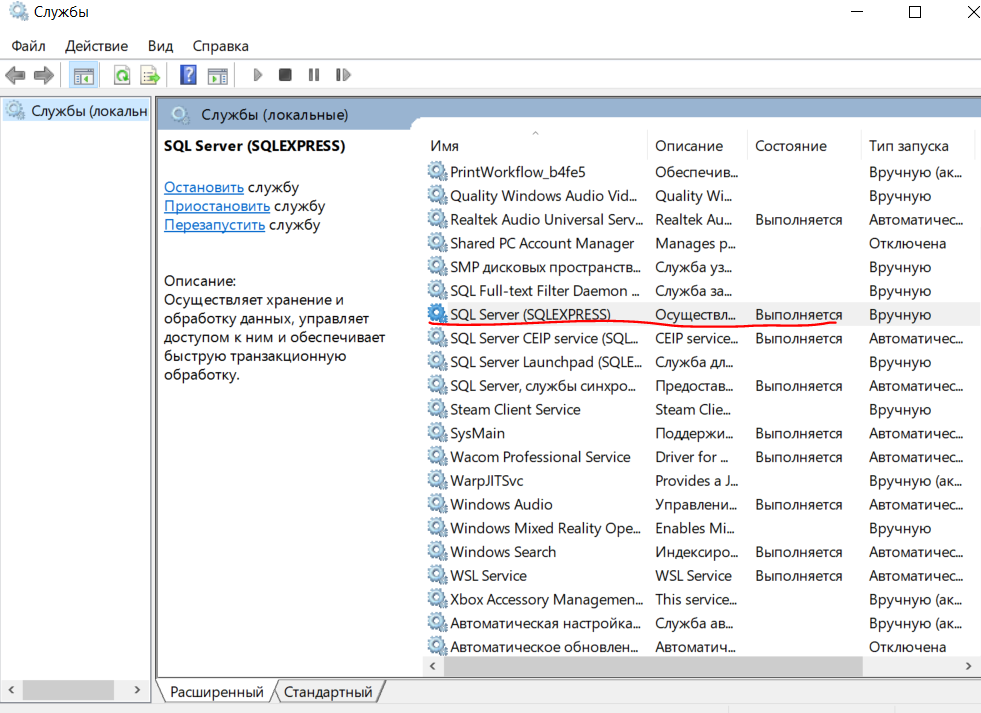
\includegraphics[width=1\linewidth]{Pic/lab1/SQLServer.PNG}
            \caption{Запуск ядра SQL.}
            \label{fig:SQLServer}
    \end{minipage}
    \hfill
    \begin{minipage}[p]{0.45\linewidth}
            \centering
            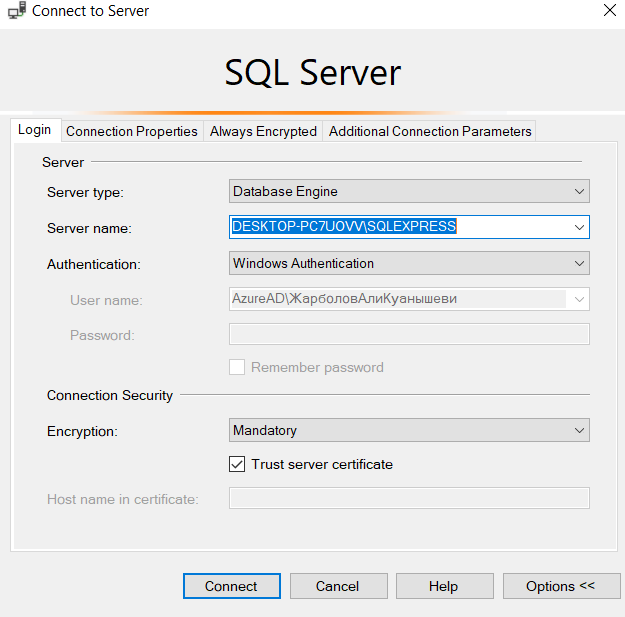
\includegraphics[width=0.8\linewidth]{Pic/lab1/SQLServerConnect.PNG}
            \caption{Подключение к локальному серверу.}
            \label{fig:Connect}
    \end{minipage}
    
\end{figure}

Если ядро запущено правильно, то соединение будет успешным. Далее необходимо создать базу данных. Это легко можно сделать через интерфейс SSMS. Выберем директорию локального сервера Database, кликнем правой кнопкой мыши и нажмём New Database. 

Далее создадим вкладку для команд (рис. \ref{fig:NewQuery}) Transact-SQL. Эти команды используются для передачи исполняемых процедур и программ на удалённый сервер. Для передачи независимых групп команд используется ключевое слово GO. 

\begin{figure}[h!]
    \centering
    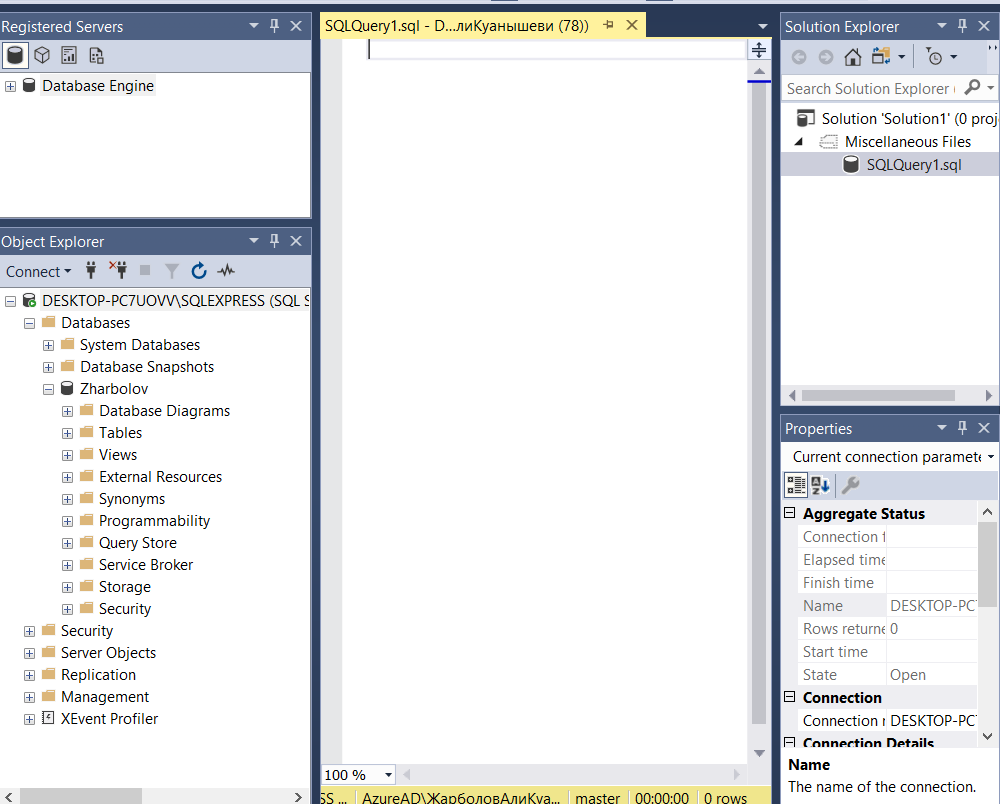
\includegraphics[width=0.3\linewidth]{Pic/lab1/NewQuery.PNG}
    \caption{Вкладка команд Transact-SQL.}
    \label{fig:NewQuery}
\end{figure}

В списке Databases обозревателя выберем созданную БД. В контекстном меню откроём её параметры (рис. \ref{fig:PROPDATABASE}), также установим её для доступа по умолчанию для команд Transact-SQL.

В открывшемся окне мы видим следующие параметры БД: Имя, владелец, дата создания, размер, колонки, доступное пространство памяти и т.п. Те же самые параметры можно получить при помощи команды Transact-SQL - sp\_helpdb. 

Заодно сразу рассмотрим команду sp\_dboption, которая проверяет значения опций созданной бд. Однако неизвестно, есть ли эта команда в нашей версии SQL Express, поэтому проверим среди встроенных процедур. Напишем следующий запрос в окне команд:

\begin{verbatim}
        USE master;
        EXEC sp_helpdb 'Zharbolov'
        GO
        select * from master.sys.sysobjects where name = 'sp_dboption'
\end{verbatim}

Вывод для команды sp\_helpdb представлен ниже, а вот выборка не вывела нам ни одного элемента, что означает отсутствие встроенной процедуры sp\_dboption. Необходимо её восстановить. Напишем и исполним следующий код восстановления. Полный код доступен в листинге (гл. \ref{CODE:sp_dboption}).

\begin{figure}[h!]
    \begin{minipage}[p]{0.45\linewidth}
        \centering
        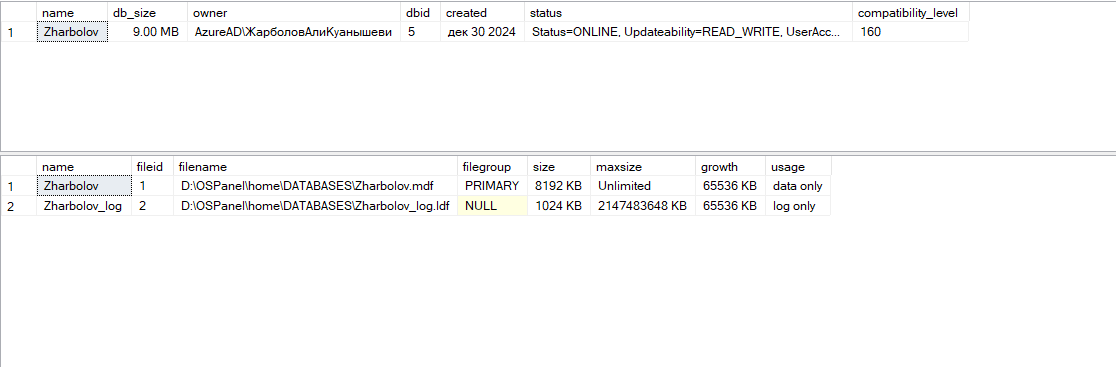
\includegraphics[width=1\linewidth]{Pic/lab1/HELP_DB.PNG}
        \caption{Вывод команды sp\_helpdb}
        \label{fig:enter-label}
    \end{minipage}
    \hfill
    \begin{minipage}[p]{0.45\linewidth}
        \centering
        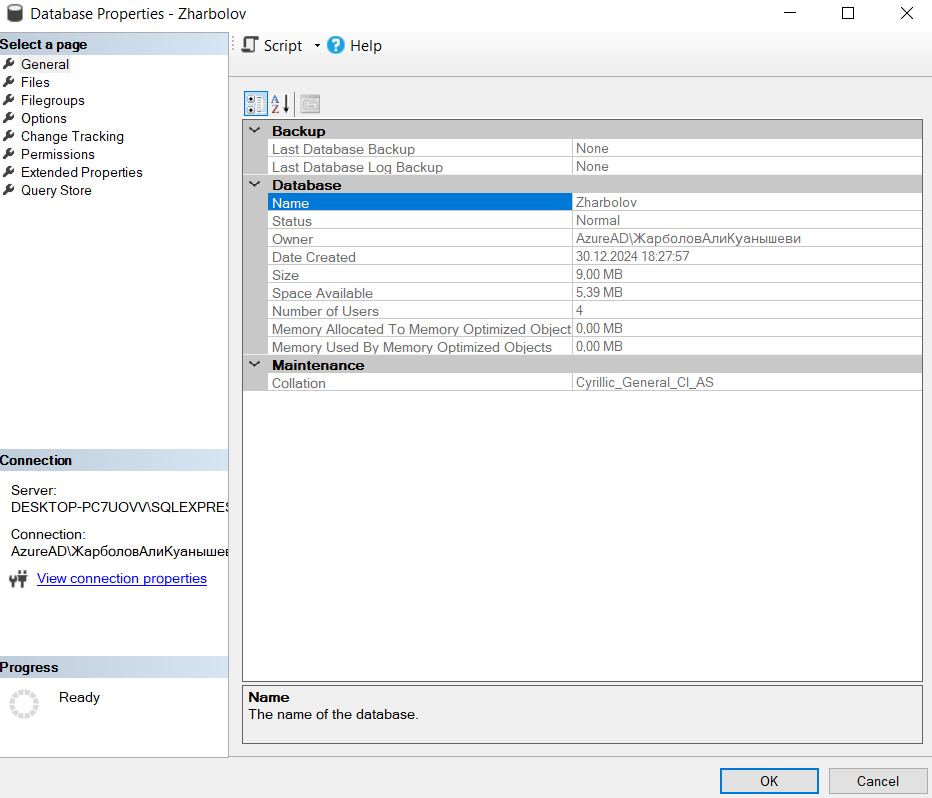
\includegraphics[width=0.45\linewidth]{Pic/lab1/DataBaseProperties.PNG}
        \caption{Параметры БД.}
        \label{fig:PROPDATABASE}
    \end{minipage}
    
\end{figure}

Теперь же наконец проверим опции нашей базы данных: 

\begin{verbatim}
        USE master
        EXEC sp_dboption 'Zharbolov', 'read only', 'TRUE'
\end{verbatim}

Далее нажимаем правой кнопкой мыши на БД в обозревателе, выбираем Script DATABASE as; CREATE to. Managament Studio создаст для нас скрипт создания базы данных(рис. \ref{fig:SCRIPTCREATEBD}).

\begin{figure}[h!]
    \centering
    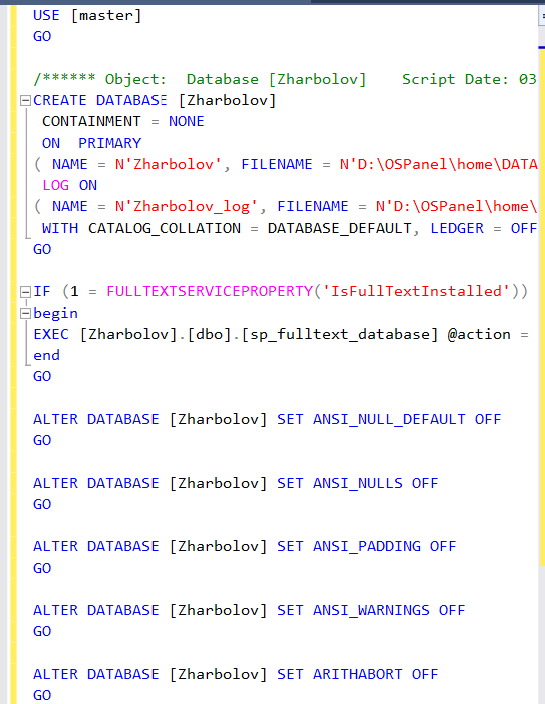
\includegraphics[width=0.5\linewidth]{Pic/lab1/SCRIPT.PNG}
    \caption{Скрипт создания базы данных.}
    \label{fig:SCRIPTCREATEBD}
\end{figure}

Здесь можно заметить основные команды для создания БД. CREATE создаёт сущность, в качестве которой мы указываем DATABASE. После чего указываем параметры БД, такие как CONTAITMENT - содержание БД; ON PRIMARY помещает бд в основную файловую группу и т.д. 

Далее указаны характеристики, которые мы видели, используя команду sp\_helpdb. И перечисляются процедуры исполнения в случае, если БД будет изменяться. Можно заметить, что команды разделены ключевым словом GO. Также используются: EXEC - исполнить; begin - начало блока команд; end - конец блока. 

Проверим скрипт. Для этого удалим БД через обозревателя (рис. \ref{fig:DBDELETE}). Потом выполним заранее созданный скрипт и проверим наличие БД по адресу $D:\backslash OSPanel\backslash home\backslash DATABASES\backslash $ (рис. \ref{fig:DBCREATE}).

\begin{figure}[h!]
    \begin{minipage}[p]{0.45\linewidth}
        \centering
        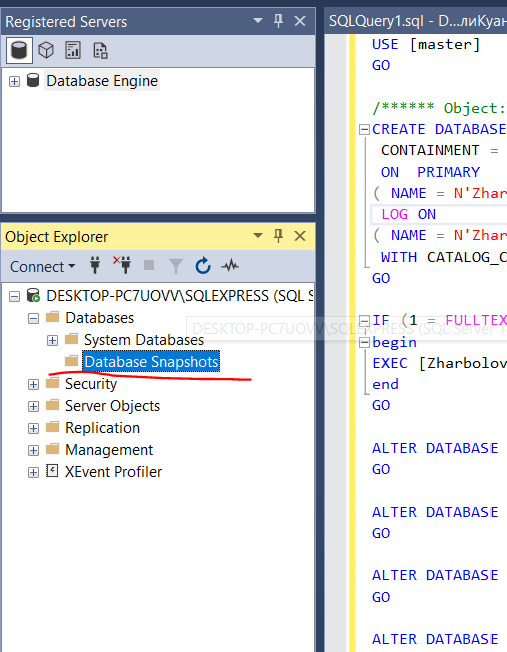
\includegraphics[width=1\linewidth]{Pic/lab1/DBDELETE.PNG}
        \caption{Удаляем базу данных.}
        \label{fig:DBDELETE}
    \end{minipage}
    \hfill
    \begin{minipage}[p]{0.45\linewidth}
        \centering
        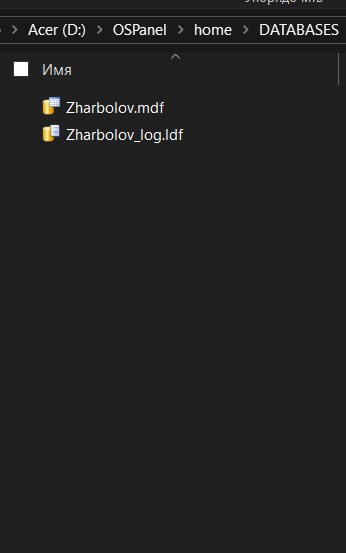
\includegraphics[width=0.82\linewidth]{Pic/lab1/DBCREATE.PNG}
        \caption{Проверяем создание базы данных}
        \label{fig:DBCREATE}
    \end{minipage}
    
\end{figure}

Теперь создадим новую таблицу через тот же обозреватель. Выбираем Tables внутри базы данных, нажимаем правой кнопкой мыши и кнопку New. Добавим в наш запрос ещё и скрипт для создания таблицы. Скрипт можно сгенерировать через обозревателя, нажав правой кнопкой мыши на таблицу, далее Script Table as; CREATE to.

\begin{verbatim}
        USE [Zharbolov]
        GO
        
        SET ANSI_NULLS ON
        GO
        
        SET QUOTED_IDENTIFIER ON
        GO
        
        CREATE TABLE [dbo].[TESTtable](
        	[NAME] [nchar](10) NULL
        ) ON [PRIMARY]
        GO
\end{verbatim}

И напишем ещё несколько команд для проверки представлений, в которых содержится наша таблица. Попробуем к тому же проверять наличие объекта с известным именем. Вывод скрипта представлен на рисунке \ref{fig:ANSTABLESCRIPT}.

\begin{verbatim}
        SELECT
          	TABLE_NAME
        FROM
          	INFORMATION_SCHEMA.TABLES
        GO
        
        SELECT
          	TABLE_NAME,
        COLUMN_NAME
        FROM
          	INFORMATION_SCHEMA.COLUMNS
        GO
        
        IF EXISTS(
        SELECT *
          		FROM
          			INFORMATION_SCHEMA.TABLES
          		WHERE
          			TABLE_NAME = 'Album'
        			)
        SELECT 'found' AS search_result ELSE 
        SELECT 'not found' AS search_result
        GO
\end{verbatim}
\begin{figure}[h!]
    \centering
    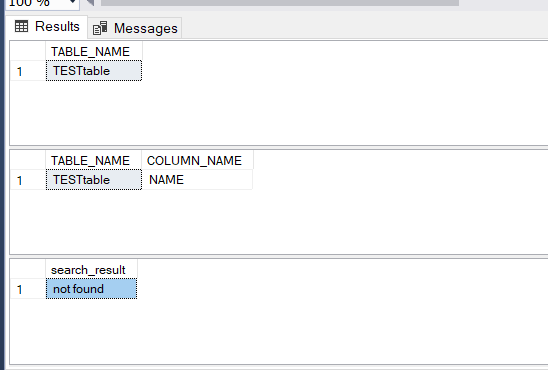
\includegraphics[width=0.5\linewidth]{Pic/lab1/ANS.PNG}
    \caption{Полученный вывод для команды к таблице.}
    \label{fig:ANSTABLESCRIPT}
\end{figure}
\subsection{Вывод}

В ходе выполнения лабораторной работы мы ознакомились с функционалом MS Management Studio. Была создана база данных, провелась настройка её параметров; внутри базы данных была создана таблица. Для каждого объекта были сгенерированы скрипты для повторного создания на других устройствах. Получены файлы с запросами.

\newpage
\section{Создание таблиц базы данных под управлением MS SQL Server}

При помощи запросов MS SQL Management Studio можно создавать таблицы, обозначая все ключи и связи. \label{LAB2}

\subsection{Цель работы}
\begin{enumerate}
    \item Изучить средства для создания и изменения структуры таблиц.
    \item Создать таблицу в базе данных из главы \ref{GL1}.
    \item Построить ER-диаграмму.
\end{enumerate}

\subsection{Ход работы}

В данной лабораторной работе мы будем создавать следующую таблицу:
\begin{figure}[h!]
    \centering
    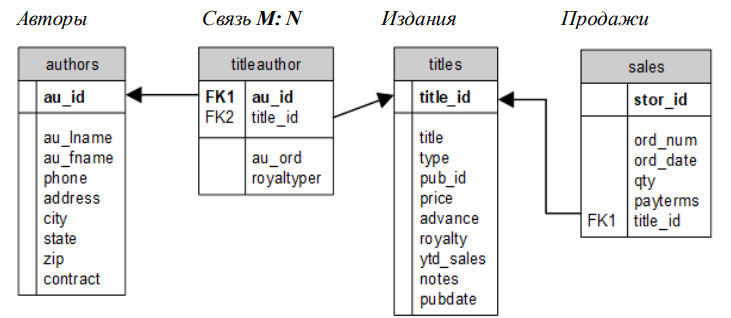
\includegraphics[width=0.5\linewidth]{Pic/lab2/Table.PNG}
    \caption{ER-диаграмма создаваемой таблицы}
    \label{fig:enter-label}
\end{figure}

База будет содержать четыре таблицы: \textbf{authors},   \textbf{titles}, \textbf{titleauthor}, \textbf{sales}. Описание таблиц, назначение колонок, тип хранимых данных и т.д. описаны в доп. информации в главе \ref{DB2INFO}. Создавать таблицу будем при помощи запросов SQL Management Studio. Сначала введём следующие команды:
\begin{verbatim}
        SET ANSI_NULLS ON
        GO

        SET QUOTED_IDENTIFIER ON
        GO
\end{verbatim}

Далее запишем скрипты для самих таблиц. Их так же можно создать через конструктор, но в таком случае нам придётся редактировать параметры созданных таблиц.

\textbf{Создание таблицы authors}
\begin{verbatim}
        CREATE TABLE [dbo].[authors](
            au_id varchar(11) CHECK (au_id like
                '[0-9][0-9][0-9]-[0-9][0-9]
                -[0-9][0-9][0-9][0-9]') 
                CONSTRAINT FK_titleauthor_1 
                PRIMARY KEY CLUSTERED,
            au_lname varchar(40) NOT NULL,
            au_fname varchar(20) NOT NULL,
            phone char(12) NOT NULL DEFAULT('UNKNOWN'),
            adress varchar(40) NULL,
            city varchar(20) NULL,
            [state] char(2) CHECK([state] like 
                '[A-Z][A-Z]') NULL,
            zip char(5) NULL CHECK (zip like '[0-9]
                [0-9][0-9][0-9][0-9]'),
            [contract] bit NOT NULL		)
\end{verbatim}
\newpage

\textbf{Создание таблицы titles}
\begin{verbatim}
        CREATE TABLE [dbo].[titles](
            title_id varchar(6) CONSTRAINT 
                FK_titleauthor_2 
                PRIMARY KEY CLUSTERED,
            title varchar(80) NOT NULL,
            [type] char(12) NOT NULL 
                DEFAULT('UNDECIDED'),
            pub_id char(4) NULL,
            price money NULL,
            advance money NULL,
            royalty int NULL,
            ytd_sales int NULL,
            notes varchar(200) NULL,
            pubdate datetime NOT NULL 
                DEFAULT(getdate()))
\end{verbatim}

\textbf{Создание таблицы titleauthor}
\begin{verbatim}
        CREATE TABLE [dbo].[titleauthor](
            au_id varchar(11) REFERENCES 
                authors(au_id),
            title_id varchar(6) REFERENCES 
                titles(title_id),
            au_ord tinyint NULL,
            royaltyper int NULL,
            CONSTRAINT PK_at1 PRIMARY KEY 
                CLUSTERED(au_id, title_id)		)
\end{verbatim}

\textbf{Создание таблицы sales}
\begin{verbatim}
        CREATE TABLE [dbo].[sales](
            stor_id char(4) NOT NULL,
            ord_num varchar(20) NOT NULL,
            ord_date datetime NOT NULL,
            qty smallint NOT NULL,
            payterms varchar(12) NULL,
            title_id varchar(6) NOT NULL	)
        GO
\end{verbatim}

Осталась последняя команда. Зададим для таблицы sales внешние ключи следующей командой:
\begin{verbatim}
        ALTER TABLE [dbo].[sales] ADD FOREIGN KEY
        ([title_id]) REFERENCES [dbo].[titles] ([title_id])
\end{verbatim}

Для создания таблиц мы использовали шаблон CREATE TABLE. Задали имя группы [dbo], и названия самих таблиц. Далее перечислили атрибуты и значения, которые они хранят. Так же использованы регулярные выражения для ограничения ввода в некоторые поля. 

Командой ALTER TABLE мы редактируем свойства таблицы, в данном случае добавляем зависимости. 

Теперь посмотрим, как выглядят связи (построим ER-диаграмму). Однако после 19 версии Management Studio эта функция устарела, так что предлагаю воспользоваться DBeaver для того, чтобы увидеть всю систему. 

Первое, что нам нужно сделать - это запустить службу обозревателя SQL Server. Иначе мы не сможем подключиться к БД из бивера.Находим в службах Windows (рис. \ref{fig:Explorer}), ставим ручной запуск и включаем службу (рис. \ref{fig:ExplorerStart}).

\begin{figure}[h!]
    \begin{minipage}[p]{0.45\linewidth}
        \centering
        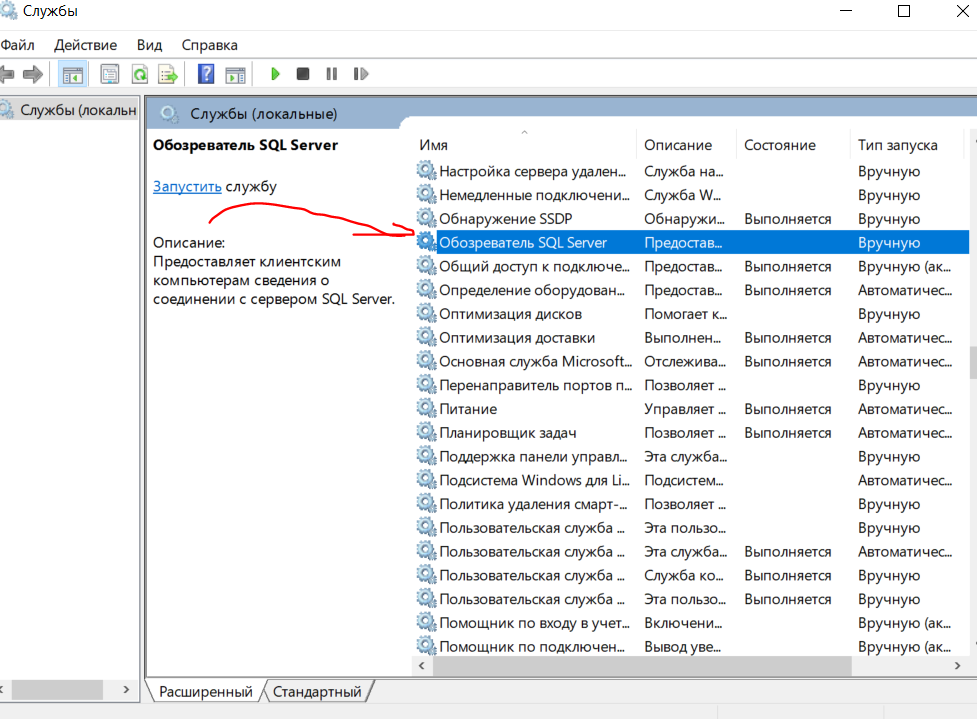
\includegraphics[width=1\linewidth]{Pic/lab2/Explorer.PNG}
        \caption{Поиск Обозревателя SQL Server.}
        \label{fig:Explorer}
    \end{minipage}
    \hfill
    \begin{minipage}[p]{0.45\linewidth}
        \centering
        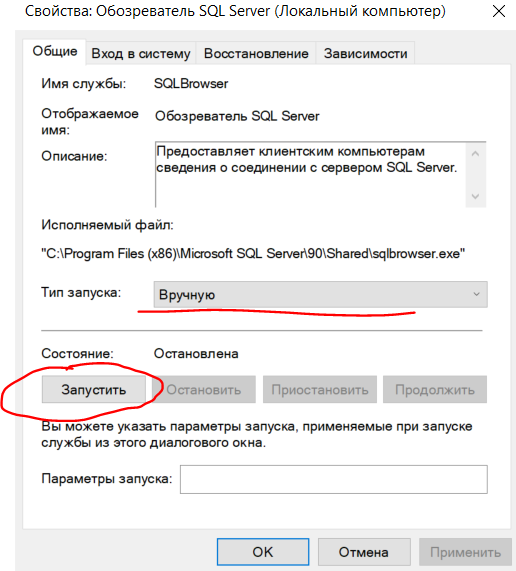
\includegraphics[width=0.68\linewidth]{Pic/lab2/ExplorerStart.PNG}
        \caption{Запуск Обозревателя}
        \label{fig:ExplorerStart}
    \end{minipage}
    
\end{figure}
\newpage
Далее необходимо разершить подключение к базе данных через SQL Server Configuration Manager (рис. \ref{fig:ConfigNet}). Внутри него надо открыть сетевые конфигурации, далее указать протоколы и разрешить подключение по TCP (рис. \ref{fig:Protocols}).

\begin{figure}[h!]
    \begin{minipage}[p]{0.45\linewidth}
        \centering
        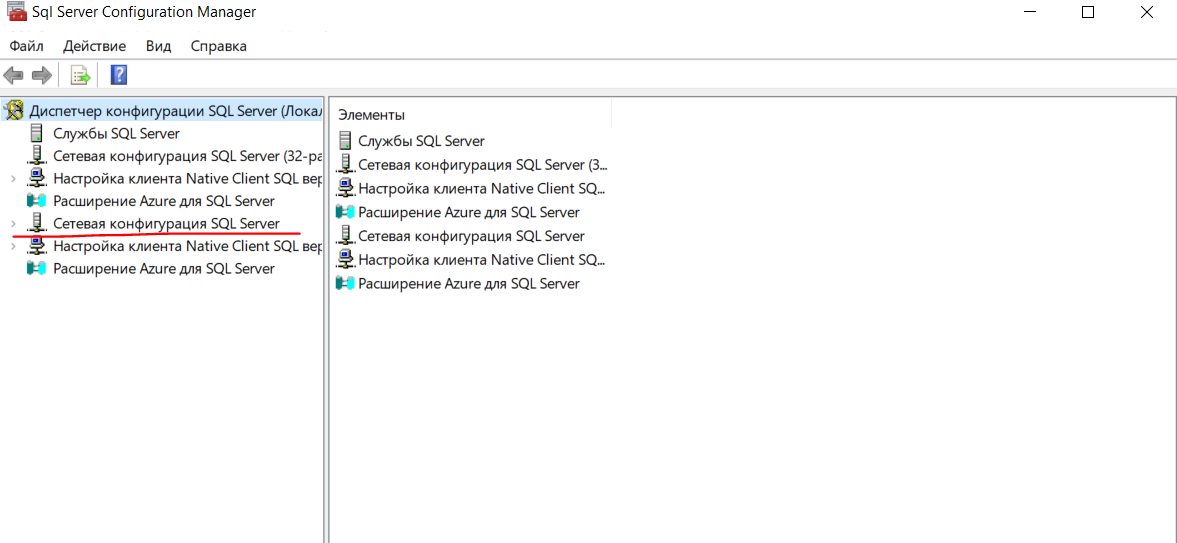
\includegraphics[width=1\linewidth]{Pic/lab2/ConfigNet.PNG}
        \caption{Поиск Обозревателя SQL Server.}
        \label{fig:ConfigNet}
    \end{minipage}
    \hfill
    \begin{minipage}[p]{0.45\linewidth}
        \centering
        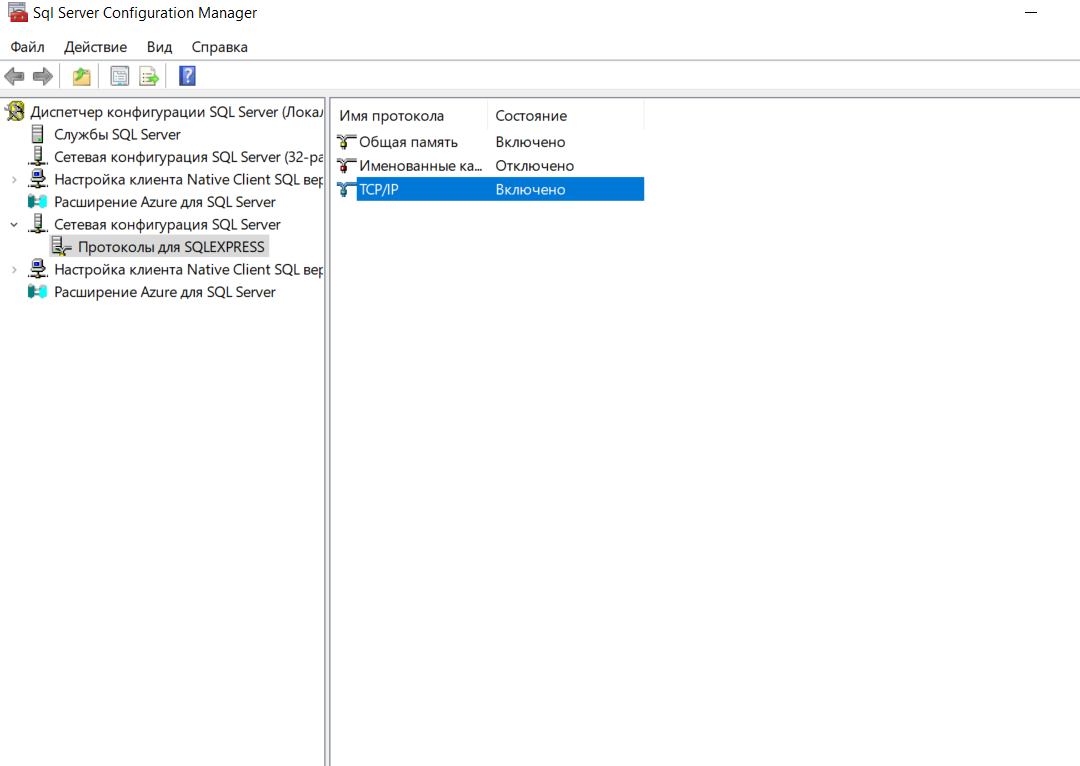
\includegraphics[width=0.68\linewidth]{Pic/lab2/Protocols.PNG}
        \caption{Запуск Обозревателя}
        \label{fig:Protocols}
    \end{minipage}
    
\end{figure}

Теперь наша БД открыта для подключения по TCP. Запускаем DBeaver, создаём новое подключение к SQL Server. Указываем имя сервера (наш компьютер), в моём случае DESKTOP-PC7UOVV$\backslash$SQLEXPRESS. Выбираем тип аутентификации Windows Authentication, подключаемся (рис. \ref{fig:ConnectBeaver}).
\begin{figure}[h!]
    \centering
    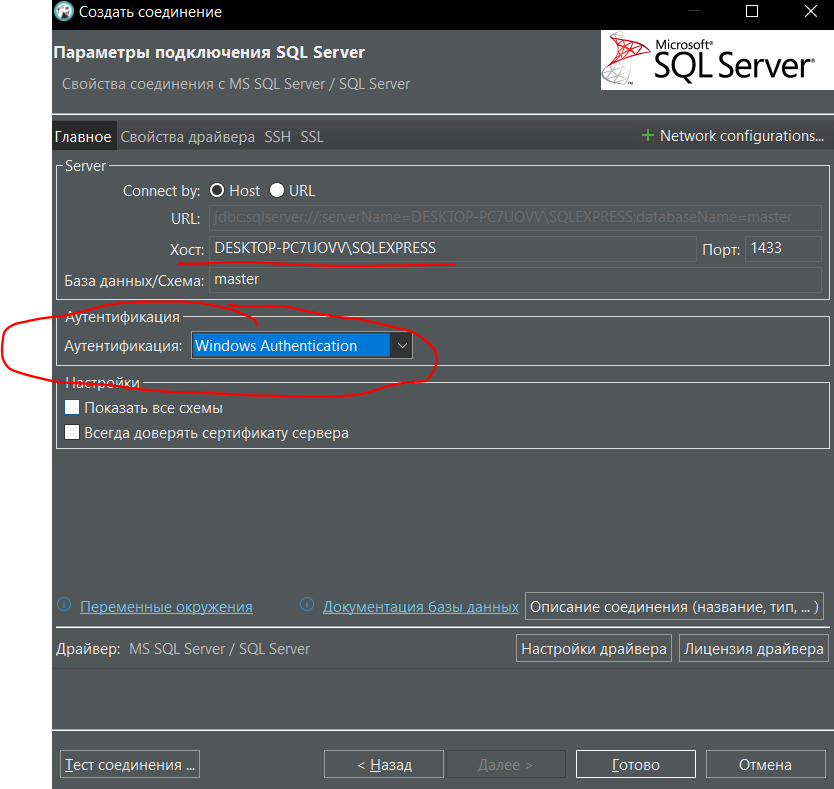
\includegraphics[width=0.5\linewidth]{Pic/lab2/ConnectBeaver.PNG}
    \caption{Подключение к БД через Beaver.}
    \label{fig:ConnectBeaver}
\end{figure}
\newpage
Открываем DataBase Diagram и видим устройство таблиц внутри БД (рис. \ref{fig:ERP}).

\begin{figure}
    \centering
    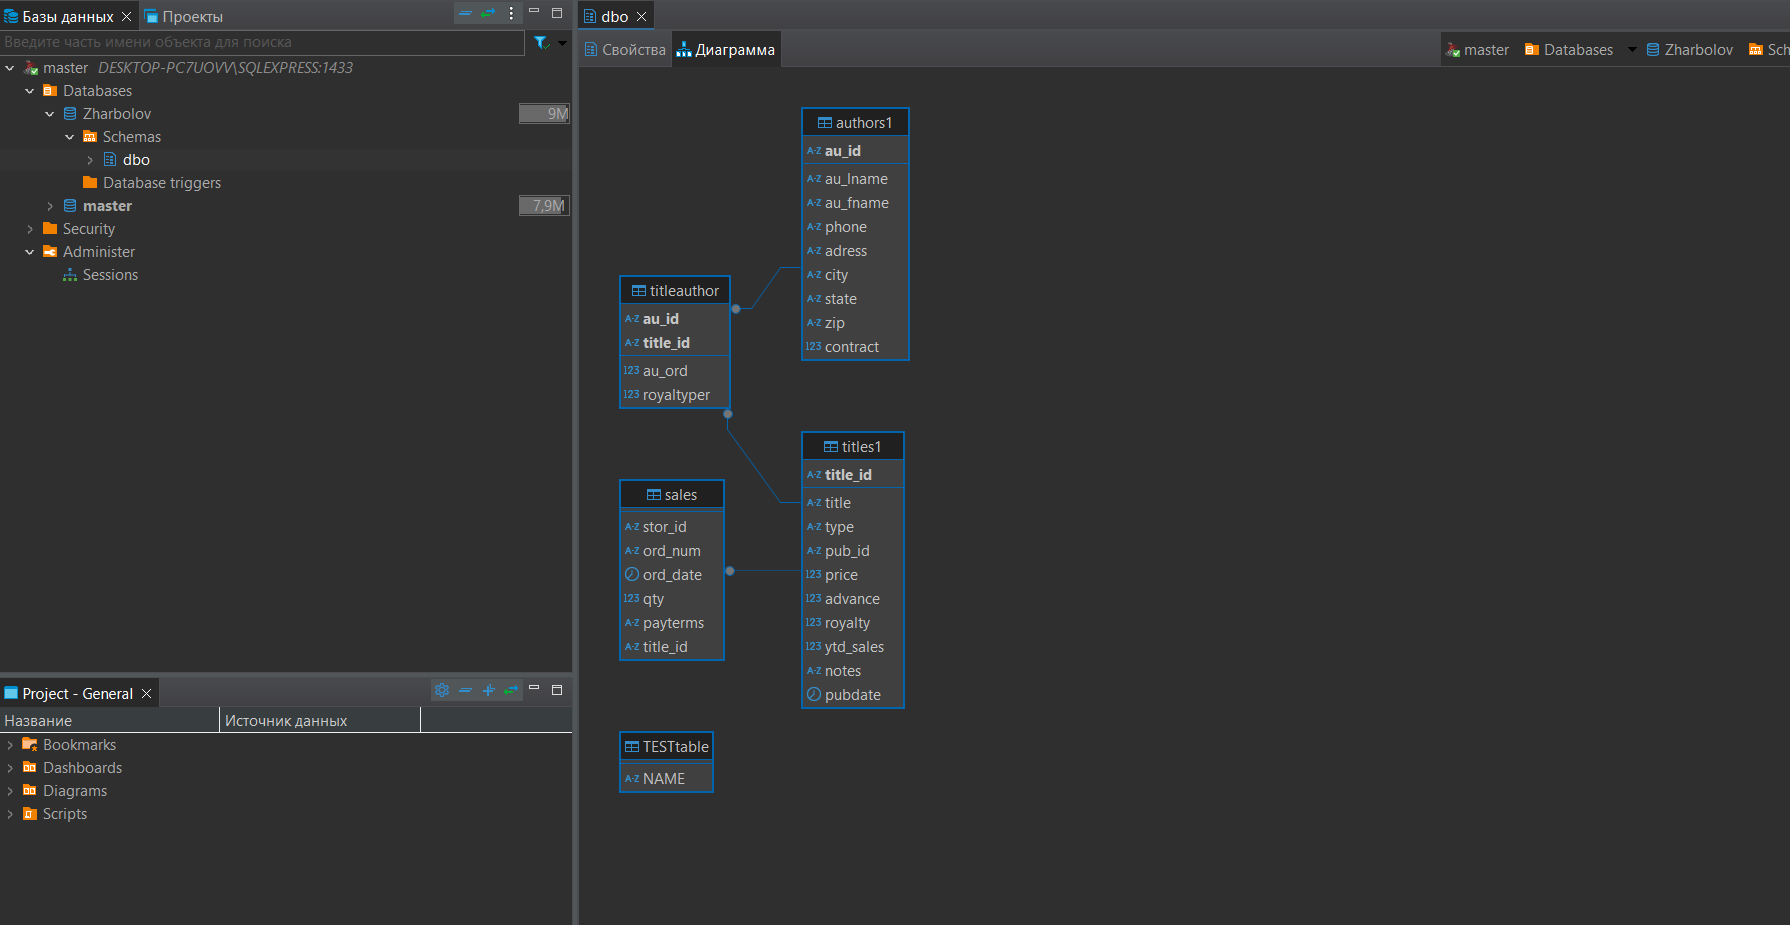
\includegraphics[width=0.8\linewidth]{Pic/lab2/ERP.PNG}
    \caption{ER-диаграмма.}
    \label{fig:ERP}
\end{figure}

Как видно из кода для создания таблиц, мы можем удалить внешние ключи, вызвав команду ALTER TABLE. Например, для таблицы titles мы можем удалить ограничение следующим образом:

\begin{verbatim}
        ALTER TABLE dbo.titles
        DROP CONSTRAINT FK_titleauthor_2;
        GO
\end{verbatim}

А вот создать обратно несколько сложнее. Ведь нам нужно указать этот ключ в той таблице, которая будет ссылаться на столбец. Создадим, допустим, из titleauthor.

\begin{verbatim}
        ALTER TABLE dpo.titleauthor
        ADD CONSTRAINT FK_titleauthor_2 FOREIGN 
            KEY (au_id) REFERENCES dbo.authors(au_id)
\end{verbatim}

Таким образом, можно добавить ключ в таблицу.

\subsection{Вывод}

В ходе работы мы изучили средства создания и изменения таблиц, их структуры и ключей. Создали в базе данных несколько таблиц и построили для них ER-диаграмму.
\newpage
\section{Загрузка таблиц базы. Передача данных между таблицами}
В таблицы из баз данных можно загружать данные из источника. Для этого существуют специальные команды transact.
\label{LAB3}
\subsection{Цель работы}
\begin{itemize}
    \item Изучить T-SQL команды INSERT, INSERT-SELECT.
    \item Внести данные из файла в базу данных.
    \item Добавить запросы данных из таблиц.
    \item Добавить с таблицы данные о книге Карпова Т. С. Базы данных: модели, разработка, реализация, 2001.
\end{itemize}
\subsection{Ход работы}
Заполним таблицы, созданные в лабораторной работе №\ref{LAB2}. Они должны соответствовать формату. Например, в таблице authors данные по книге Понамарёва В. "Базы данных в Delphi 7. Самоучитель" могут быть представлены так:
\begin{verbatim}
            | 123-12-1234 
            | Понамарёв 
            | Вячеслав _89121234567 
            | ул. Вишнёвая д. 12, кв. 31 
            | Екатеринбург 
            | РФ 12345 
            | 1
\end{verbatim}
Выполним вставку данных в таблицу authors (рис. \ref{fig:FQ12}). На рисунке выделяется синтаксическая ошибка, однако она связана с тем, что SQL Manager не видит обновление БД без перезапуска SQL Сервера.
\begin{verbatim}
    INSERT authors VALUES('111-00-0004', 'Алексей', 'Хохлов'...
    INSERT authors VALUES('409-56-7008', 'Bennet', 'Abraham'...
    INSERT authors VALUES('213-46-8915', 'Green', 'Marjorie'...
    INSERT authors VALUES('238-95-7766', 'Carson', 'Cheryl'...
    INSERT authors VALUES('111-00-0001', 'Игорь', 'Фигурнов'...
    INSERT authors VALUES('998-72-3567', 'Ringer', 'Albert'...
    INSERT authors VALUES('899-46-2035', 'Ringer', 'Anne'...
    INSERT authors VALUES('111-00-0002', 'Сергей', 'Каратыгин'...
    
    INSERT authors VALUES('722-51-5454', 'DeFrance', 'Michel'...
    ('807-91-6654', 'Panteley', 'Sylvia'...
    ('893-72-1158', 'McBadden', 'Heather'...
    ('724-08-9931', 'Stringer', 'Dirk'...
    ('274-80-9391', 'Straight', 'Dean'...
    ('756-30-7391', 'Karsen', 'Livia'...
    ('724-80-9391', 'MacFeather', 'Stearns'...
    ('427-17-2319', 'Dull', 'Ann'...
    ('672-71-3249', 'Yokomoto', 'Akiko'...
    ('267-41-2394', 'O''Leary', 'Michael'...
    ('472-27-2349', 'Gringlesby', 'Burt'...
    ('527-72-3246', 'Greene', 'Morningstar'...
    ('172-32-1176', 'White', 'Johnson'...
    ('712-45-1867', 'del Castillo', 'Innes'...
    ('846-92-7186', 'Hunter', 'Sheryl'...
    ('486-29-1786', 'Locksley', 'Charlene'...
    ('648-92-1872', 'Blotchet-Halls', 'Reginald'...
    ('341-22-1782', 'Smith', 'Meander'...
    GO
\end{verbatim}
\begin{figure}[h!]
    \centering
    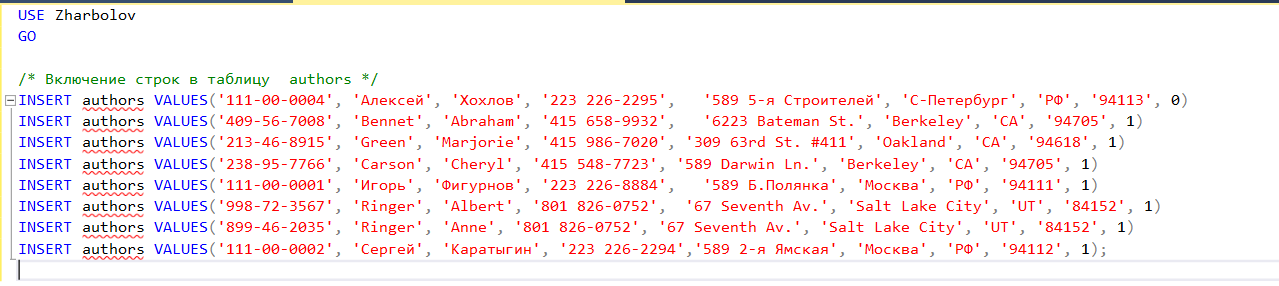
\includegraphics[width=0.8\linewidth]{Pic/lab3/FQ1.PNG}
    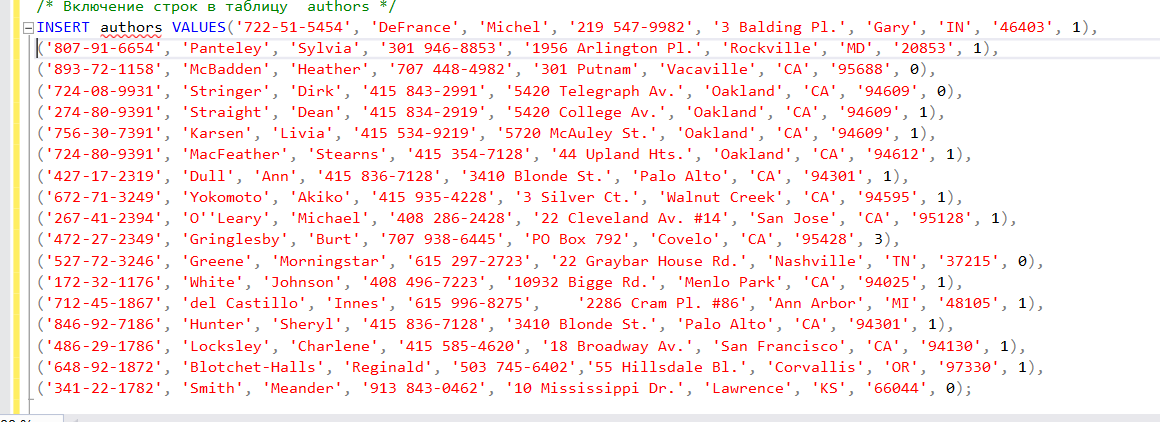
\includegraphics[width=0.8\linewidth]{Pic/lab3/FQ2.PNG}
    \caption{Запрос на вставку в таблицу authors.}
    \label{fig:FQ12}
\end{figure}

Выполним вставку данных в таблицу в titles (рис. \ref{fig:TQ12}). На рисунках выделяется та же синтаксическая ошибка. 

\begin{verbatim}
        INSERT titles VALUES ('PC1111', 'Популярно...
        INSERT titles VALUES ('PC8888', 'Secrets...
        INSERT titles VALUES ('BU1032', 'The Busy...
        INSERT titles VALUES ('PS7777', 'Emotional...
        INSERT titles VALUES ('PS3333', 'Prolonged...
        INSERT titles VALUES ('BU1111', 'Cooking...
        INSERT titles VALUES ('MC2222', 'Silicon...
        INSERT titles VALUES ('TC7777', 'Sushi...
        INSERT titles VALUES ('TC4203', 'Fifty...
        INSERT titles VALUES ('PC1035', 'But...
        INSERT titles VALUES('BU2075', 'You...
        INSERT titles VALUES('PS2095', 'Is Anger...
        INSERT titles VALUES('PS2106', 'Life Without...
        INSERT titles VALUES('MC3021', 'The Gourmet...
        INSERT titles VALUES('TC3219', 'Onions...
        INSERT titles (title_id, title, pub_id) 
            VALUES('MC3026', 'The Psychology...
        INSERT titles VALUES ('BU7832', 'Straight Talk...
        INSERT titles VALUES('PS1372', 'Computer Phobic...
        INSERT titles (title_id, title, type, pub_id, notes) 
            VALUES('PC9999', 'Net Etiquette'...
        INSERT titles VALUES ('PC8888', 'Secrets of...
        GO
\end{verbatim}

\begin{figure}[h!]
    \centering
    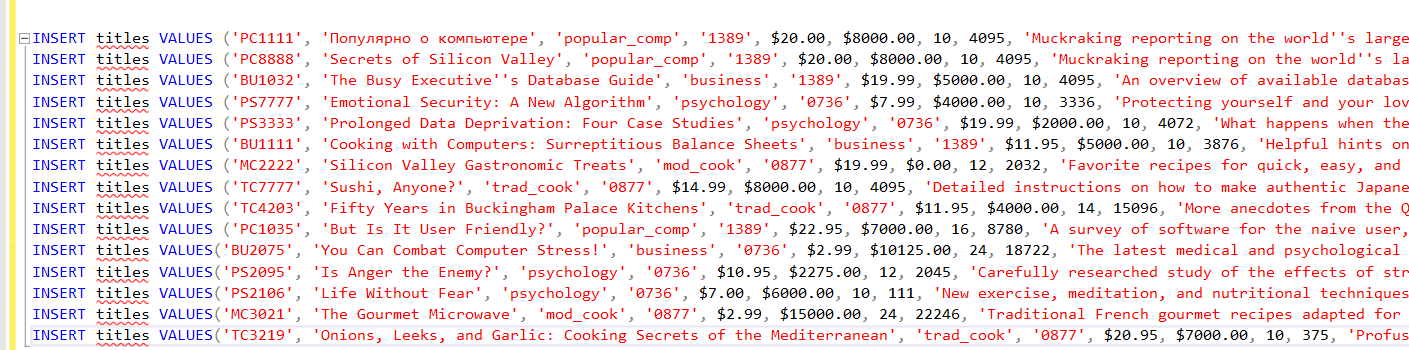
\includegraphics[width=0.8\linewidth]{Pic/lab3/TQ1.PNG}
    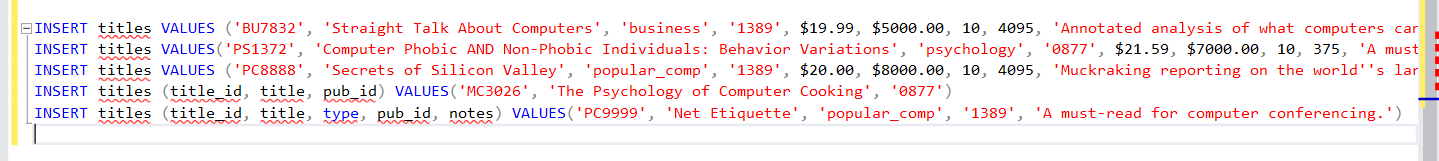
\includegraphics[width=0.8\linewidth]{Pic/lab3/TQ2.PNG}
    \caption{Запрос на вставку в таблицу titles.}
    \label{fig:TQ12}
\end{figure}

После запуска запроса происходит ошибка (рис. \ref{fig:ERR}). В том, что неверно указан формат даты - mm/dd/yy вместо dd/mm/yy (рис. \ref{fig:TQ1Solve}). Меняем форматы дат, и делаем повторную загрузку. Сделаем вставку для таблицы titleauthors (в ней тоже допущены ошибки в датах, исправление которых подробно описывать не станем).
\begin{verbatim}
        INSERT titleauthor VALUES('111-00-0004', 'PC2222', 1, 100)
        INSERT titleauthor VALUES('409-56-7008', 'BU1032', 1, 60)
        INSERT titleauthor VALUES('486-29-1786', 'PS7777', 1, 100)
        INSERT titleauthor VALUES('486-29-1786', 'PC9999', 1, 100)
        INSERT titleauthor VALUES('712-45-1867', 'MC2222', 1, 100)
        INSERT titleauthor VALUES('172-32-1176', 'PS3333', 1, 100)
        INSERT titleauthor VALUES('213-46-8915', 'BU1032', 2, 40)
                                ...
\end{verbatim}
\begin{figure}[h!]
    \centering
    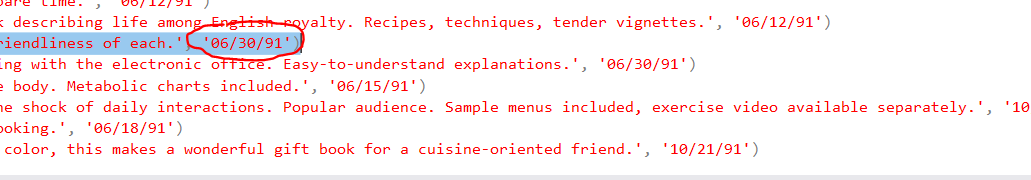
\includegraphics[width=0.8\linewidth]{Pic/lab3/TQ1Solve.PNG}
    \caption{Неверный формат дат.}
    \label{fig:TQ1Solve}
\end{figure}
\begin{figure}[h!]
    \centering
    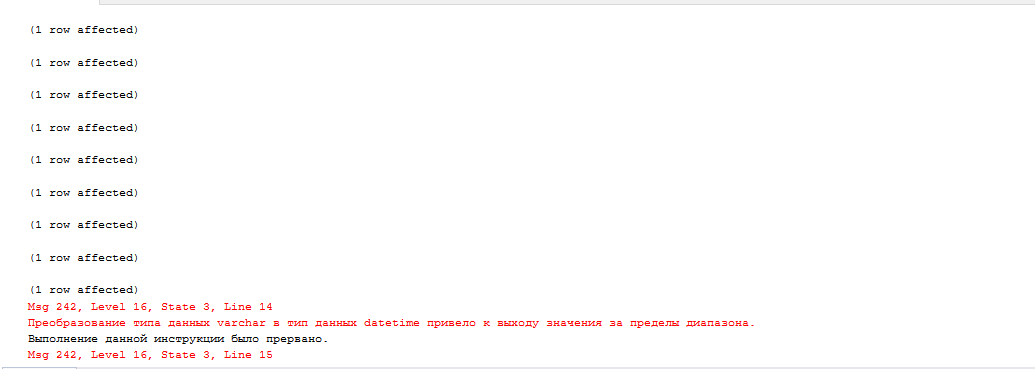
\includegraphics[width=0.85\linewidth]{Pic/lab3/TQ1ERROR.PNG}
    \caption{Ошибка вставки.}
    \label{fig:ERR}
\end{figure}

При вставке в таблицу titleauthor возникает ещё одна ошибка: не соответствие значений колонки title\_id первичному ключу. 
\begin{figure}[h!]
    \centering
    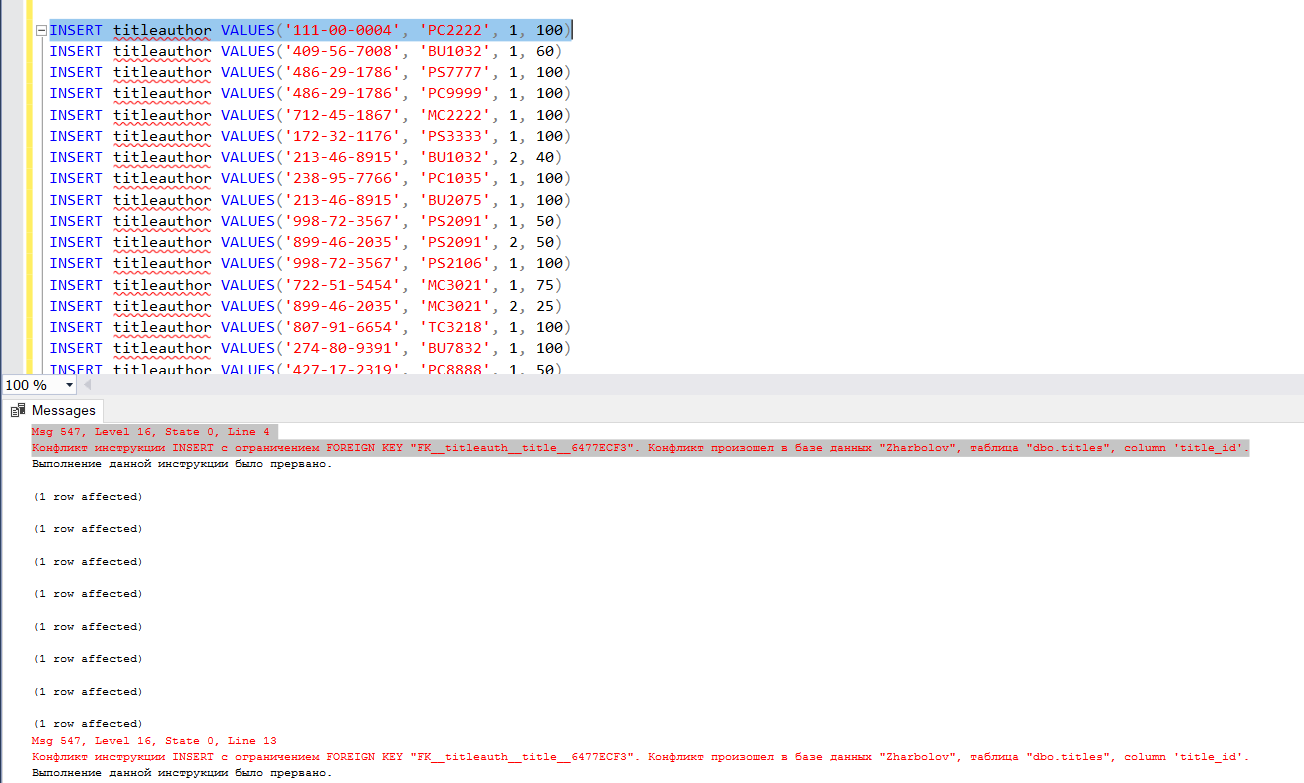
\includegraphics[width=0.7\linewidth]{Pic/lab3/TAQ1Error.PNG}
    \caption{Несоответствие значений ключу.}
    \label{fig:enter-label}
\end{figure}

Если посмотреть на возможные ключи в таблице titles через DBeaver, можно увидеть, что такие id отсутствуют (рис. \ref{fig:TAQ1ES}). Мы пытались решить противоречия самостоятельным соотнесением ключей, но, к сожалению, не удалось, соответственно строчки были удалены. 
\begin{figure}[h!]
    \centering
    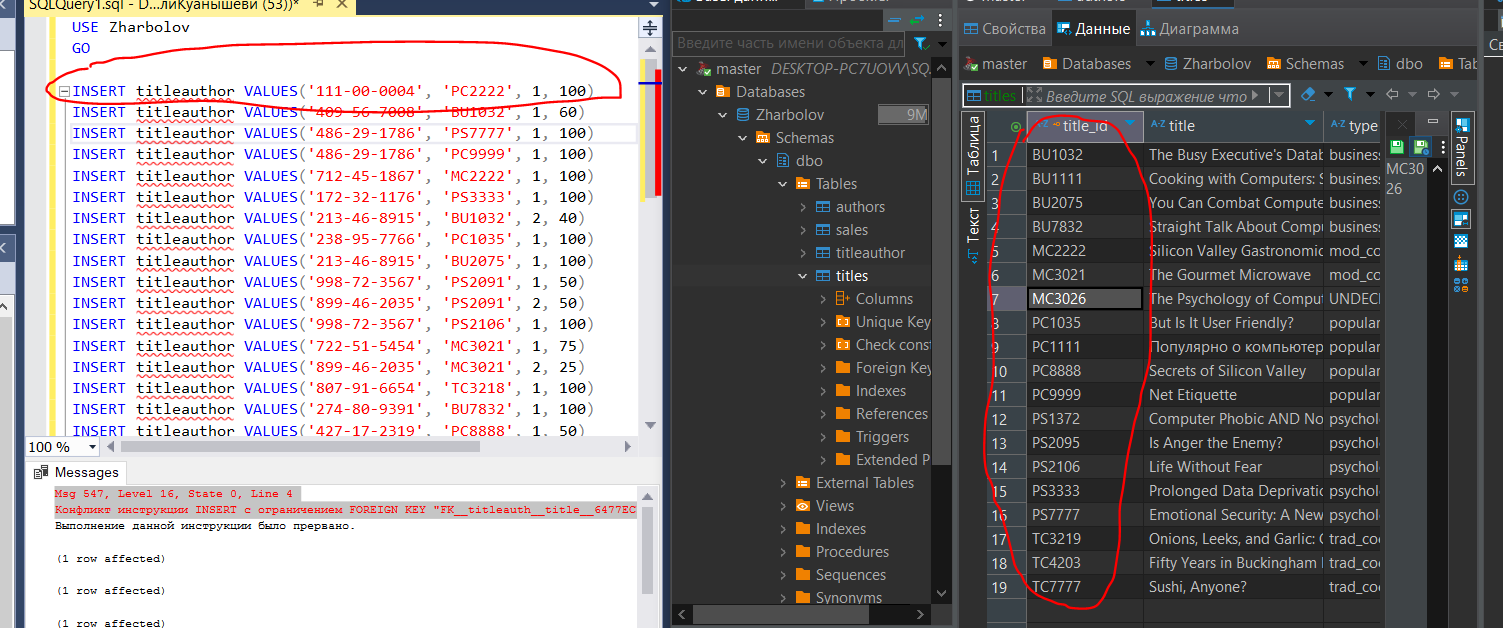
\includegraphics[width=\linewidth]{Pic/lab3/TAQ1ESolve.PNG}
    \caption{Поиск ключей в базе.}
    \label{fig:TAQ1ES}
\end{figure}

Выполним ещё один запрос для таблицы sales (даты исправлены):
\begin{verbatim}
        INSERT sales VALUES('7066', 'QA7442.3', '13/09/94', 75...
        INSERT sales VALUES('7067', 'D4482', '14/09/94', 10...
        INSERT sales VALUES('7131', 'N914008', '14/09/94', 20...
        INSERT sales VALUES('7131', 'N914014', '14/09/94', 25...
        INSERT sales VALUES('8042', '423LL922', '14/09/94', 15...
        INSERT sales VALUES('8042', '423LL930', '14/09/94', 10...
        INSERT sales VALUES('6380', '722a', '13/09/94', 3...
        INSERT sales VALUES('6380', '6871', '14/09/94', 5...
        INSERT sales VALUES('8042','P723', '11/03/93', 25...
        INSERT sales VALUES('7896','X999', '21/02/93', 35...
        INSERT sales VALUES('7896','QQ2299', '28/10/93', 15...
        INSERT sales VALUES('7896','TQ456', '12/12/93', 10...
        INSERT sales VALUES('8042','QA879.1', '22/5/93'...
        INSERT sales VALUES('7066','A2976', '24/05/93', 50...
        INSERT sales VALUES('7131','P3087a', '29/05/93', 20...
        INSERT sales VALUES('7131','P3087a', '29/05/93', 25...
        INSERT sales VALUES('7131','P3087a', '29/05/93', 15...
        INSERT sales VALUES('7131','P3087a', '29/05/93', 25...
        INSERT sales VALUES('7067','P2121', '15/06/92', 40...
        INSERT sales VALUES('7067','P2121', '15/06/92', 20...
        INSERT sales VALUES('7067','P2121', '15/06/92', 20...
\end{verbatim}

Вставку данных в таблицы можно проверить в дополнительной информации в главе \ref{DATA3}. Теперь скопируем записи из таблицы authors, где в графе штат стоит "UT". 
\begin{verbatim}
        USE Zharbolov
        GO
        CREATE TABLE QUEST3
        (
        au_id varchar(11),
        au_lname varchar(40) NOT NULL,
        au_fname varchar(20) NOT NULL,
        phone char(12) NOT NULL DEFAULT('UNKNOWN'),
        adress varchar(40) NULL,
        city varchar(20) NULL,
        [state] char(2),
        zip char(5),
        [contract] bit NOT NULL	
        );
        
        INSERT INTO QUEST3 SELECT * FROM authors WHERE [state] = 'UT'
\end{verbatim}

Проверим, что данные были скопированы в DBeaver (рис \ref{fig:DataCopy3}). Если же мы попробуем дополнить этими данными таблицу authors, ничего не получится: SQL не примет данные из-за совпадающим первичных ключей. 
\begin{figure}
    \centering
    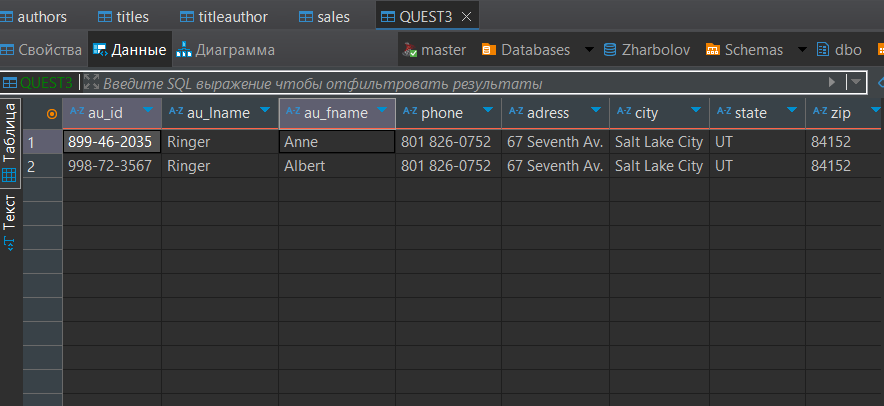
\includegraphics[width=0.9\linewidth]{Pic/lab3/DataCopy.PNG}
    \caption{Скопированные данные из таблицы authors.}
    \label{fig:DataCopy3}
\end{figure}
Теперь выведем все данные в одной таблице. Для этого последовательно начнём объединять таблицы.

\begin{verbatim}
        CREATE TABLE TABLES
        (
        au_id varchar(11),
        au_lname varchar(40) NOT NULL,
        au_fname varchar(20) NOT NULL,
        phone char(12) NOT NULL DEFAULT('UNKNOWN'),
        adress varchar(40) NULL,
        city varchar(20) NULL,
        [state] char(2),
        zip char(5),
        [contract] bit NOT NULL,	
        au_id1 varchar(11),
        title_id varchar(6),
        au_ord tinyint NULL,
        royaltyper int NULL,
        );
        
        INSERT INTO TABLES SELECT * 
        FROM authors INNER JOIN titleauthor 
        ON authors.au_id = titleauthor.au_id
\end{verbatim}

Присоединим вторую таблицу.

\begin{verbatim}
        CREATE TABLE TABLES2
        (
        au_id varchar(11),
        au_lname varchar(40) NOT NULL,
        au_fname varchar(20) NOT NULL,
        phone char(12) NOT NULL DEFAULT('UNKNOWN'),
        adress varchar(40) NULL,
        city varchar(20) NULL,
        [state] char(2),
        zip char(5),
        [contract] bit NOT NULL,
                    ...
        INSERT INTO TABLES1 SELECT * 
        FROM TABLES INNER JOIN titles
        ON TABLES.title_id = titles.title_id
\end{verbatim}

И наконец третью таблицу:

\begin{verbatim}
                    ...
        INSERT INTO TABLES2 SELECT * 
        FROM TABLES1 INNER JOIN sales
        ON TABLES1.title_id = sales.title_id
\end{verbatim}

Теперь посмотрим (результат на рисунке \ref{fig:INNERDATA}) на объединённые строчки наших таблиц следующей командой:

\begin{verbatim}
        USE Zharbolov
        GO
        
        SELECT * FROM TABLES2
\end{verbatim}

\begin{figure}[h!]
    \centering
    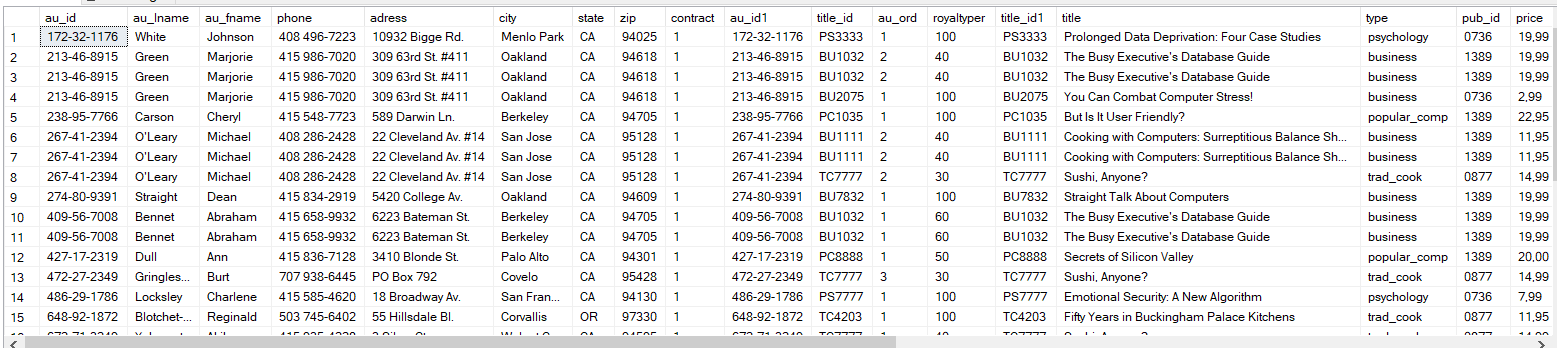
\includegraphics[width=0.9\linewidth]{Pic/lab3/INNERDATA.PNG}
    \caption{Объединённые строчки четырёх таблиц.}
    \label{fig:INNERDATA}
\end{figure}

Осталось только выполнить дополнительное задание: добавим в таблицу данные по книге Карпова Т. С. 
\begin{verbatim}
        INSERT INTO authors(au_id, au_lname, au_fname, [contract]) 
            VALUES('000-00-0000', 'Т...', 'Карпов', 1)
        INSERT INTO titles(title_id, title, [type], pubdate) 
            VALUES('KP0000', 'Базы данных: модели, разработка, 
            реализация', 'popular_comp', '01/01/01')
        INSERT INTO titleauthor(au_id, title_id) 
            VALUES('000-00-0000', 'KP0000')
        INSERT INTO sales VALUES('0001', 'KP8732', 
            '20/10/01', 75, 'ON invoice', 'KP0000')
        INSERT INTO sales VALUES('0001', 'KP8732', 
            '21/11/01', 75, 'ON invoice', 'KP0000')
        INSERT INTO sales VALUES('0001', 'KP8732', 
            '22/12/01', 75, 'ON invoice', 'KP0000')
\end{verbatim}
\subsection{Вывод}
В ходе выполнения данной лабораторной работы мы изучили команды INSERT, SELECT. Внесли данные из файла в базу данных. Написали запросы данных из таблиц и выполнили дополнительное задание. 

\section{Построение простых SQL-запросов}
в этой лабораторной работе мы напишем несколько SQL-запросов в базу данных

\subsection{Цель работы}
\begin{itemize}
    \item Добавить запросы для поиска данных в БД.
    \item Добавить запросы для выбора атрибутов таблиц.
\end{itemize}
\subsection{Ход работы}
Выполним Select-операторы для нашей БД. Для начала укажем область видимости.
\begin{verbatim}
        USE Zharbolov
\end{verbatim}

Далее выполним простейший запрос информации из нескольких столбцов.

\begin{verbatim}
        SELECT au_id, au_lname, au_fname FROM authors
\end{verbatim}

\begin{figure}[h!]
    \centering
    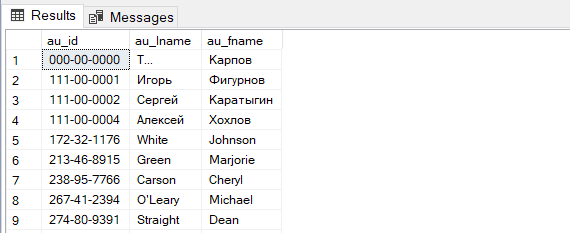
\includegraphics[width=0.9\linewidth]{Pic/lab4/SQ1.PNG}
    \caption{Простейшая SELECT-конструкция.}
    \label{fig:SELECT1}
\end{figure}

Командой SELECT мы делаем выборку из таблицы, в качестве критериев указываем нужные столбцы. Ключевое слово FROM указывает на таблицу (рис. \ref{fig:SELECT1}). Мы также можем вывести нужные нам названия столбцов, указав их в атрибуты таблицы (рис. \ref{fig:sin1}).

\begin{verbatim}
        SELECT 'идентификатор'=au_id, 'Имя' = au_lname, 'Фамилия' = au_fname
        FROM authors
\end{verbatim}

Можно сделать это и другим способом. Вместо внутренних названий атрибутов таблицы поставим удобные для чтения с помощью ключевого слова AS (рис. \ref{fig:sin2}).

\begin{verbatim}
        SELECT 
        au_id AS 'Номер', 
        au_lname AS 'Имя', 
        au_fname AS'Фамилия' 
        FROM authors  
\end{verbatim}
\begin{figure}[h!]
    \begin{minipage}[p]{0.45\linewidth}
        \centering
        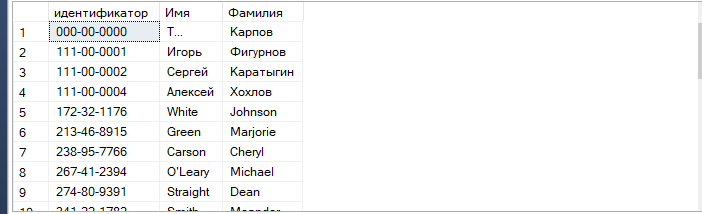
\includegraphics[width=\linewidth]{Pic/lab4/SQ2.PNG}
        \caption{Первый синтаксис для именования столбцов.}
        \label{fig:sin1}
    \end{minipage}
    \hfill
    \begin{minipage}[p]{0.45\linewidth}
        \centering
        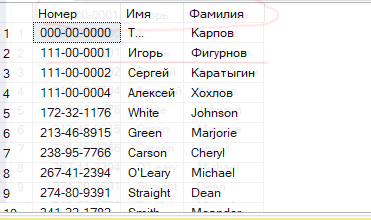
\includegraphics[width=0.55\linewidth]{Pic/lab4/SQ3.PNG}
        \caption{Второй синтаксис для именования столбцов.}
        \label{fig:sin2}
    \end{minipage}
    
\end{figure}

Можно указывать конкретные значения, которые мы ищем в базе данных. Для этого используется конструкция WHERE (рис. \ref{fig:WHEREC}).

\begin{verbatim}
        SELECT 'идентификатор'=au_id, 'Имя' = au_lname, 'Фамилия' = au_fname
        FROM authors WHERE city = 'Oakland'
\end{verbatim}
\begin{figure}[h!]
    \centering
    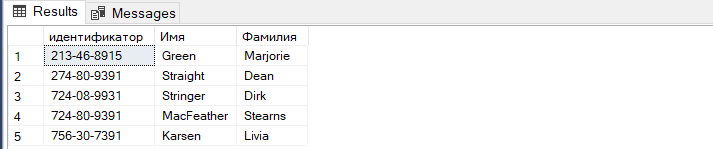
\includegraphics[width=0.9\linewidth]{Pic/lab4/SQ4.PNG}
    \caption{Использование WHERE.}
    \label{fig:WHEREC}
\end{figure}

При помощи подобного синтаксиса можно получать производные атрибуты (рис. \ref{fig:Catrib}), наподобии того, как это работает в Numpy, Pandas. Давайте выполним это для таблицы titles:

\begin{verbatim}
        SELECT title_id, price, new_price=price*1.15
        FROM titles WHERE advance !< '$5000'
\end{verbatim}

Здесь мы создали новый атрибут new\_price из атрибута price. Но, конечно, существует этот атрибут только в пространстве SQL-запроса. Мы могли бы добавить его в таблицу с помощью дополнительных запросов.

Важно, что производный атрибут даже не именован. Рассмотрим следующие команды. 

\begin{verbatim}
        SELECT title_id, ytd_sales, '2*ytd' = 2*ytd_sales
        FROM titles
\end{verbatim}
\begin{figure}[h!]
    \centering
    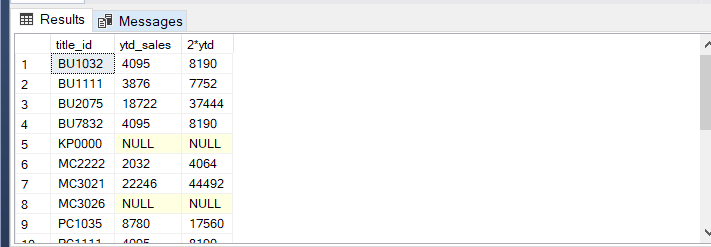
\includegraphics[width=0.9\linewidth]{Pic/lab4/SQL5.PNG}
    \caption{Формирование производного атрибута.}
    \label{fig:Catrib}
\end{figure}
Здесь прекрасно видно то, о чём мы говорили. Появилась новая колонка. Однако взглянем на следующую команду.

\begin{verbatim}
        SELECT title_id, ytd_sales, price*ytd_sales
        FROM titles
\end{verbatim}
\begin{figure}
    \centering
    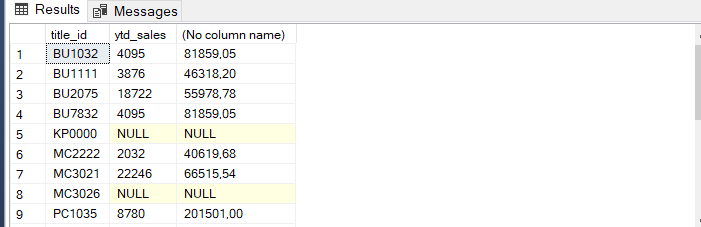
\includegraphics[width=0.9\linewidth]{Pic/lab4/SQL6.PNG}
    \caption{Формирование производного неименованного атрибута.}
    \label{fig:CatribNo}
\end{figure}

Новый атрибут на рисунке \ref{fig:CatribNo} появился, но он не именован (No column name). Ведь мы не указывали для него имя. Также удобно использовать псевдоним для таблицы, чтобы не указывать её полное название.

\begin{verbatim}
        SELECT 
        id = a.au_id, 
        fullname = a.au_lname, 
        name = a.au_fname,
        phone = a.phone,
        adress = a.adress,
        city = a.city,
        state = a.state,
        number = a.zip,
        'Is on contract?' = a.contract
        FROM authors a
\end{verbatim}

Если же мы не желаем ограничивать выдачу данных, то есть хотим получить полную таблицу, можно использовать * как в регулярных выражениях. 

\begin{verbatim}
        SELECT * FROM titles
        SELECT * FROM authors
\end{verbatim}

\begin{figure}[h!]
    \centering
    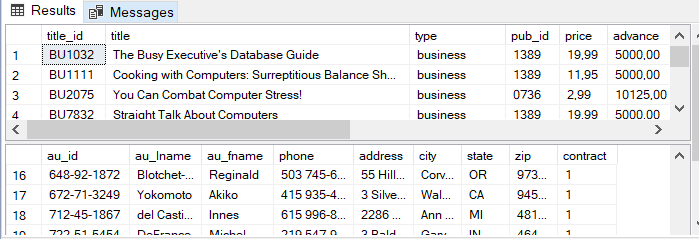
\includegraphics[width=0.9\linewidth]{Pic/lab4/SQ7.PNG}
    \caption{Получение полных таблиц.}
    \label{fig:ALLDATA}
\end{figure}

При помощи подобных команд мы можем и объединять таблицы. Правда, это может приводить к ошибках в данных (поля NULL возникают) и к дублированию строчек, если атрибуты соотносятся один ко многим (а у нас именно так)

\begin{verbatim}
        SELECT * FROM titles, sales
\end{verbatim}
\begin{figure}[h!]
    \centering
    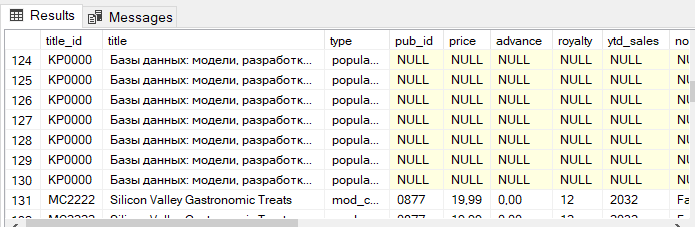
\includegraphics[width=0.9\linewidth]{Pic/lab4/SQ8.PNG}
    \caption{Совмещение двух таблиц.}
    \label{fig:enter-label}
\end{figure}

Исправить это можно уточнением запросов. Дополним предыдущую команду запросом сравнения первичного ключа со значениями title\_id таблицы sales через конструкцию WHERE и потребуем выдать результат лишь для одного id - PS2106 (рис. \ref{fig:SQ9}).

\begin{verbatim}
        SELECT * FROM titles, sales
        WHERE titles.title_id = sales.title_id 
        AND titles.title_id = 'PS2106'
\end{verbatim}
\begin{figure}[h!]
    \centering
    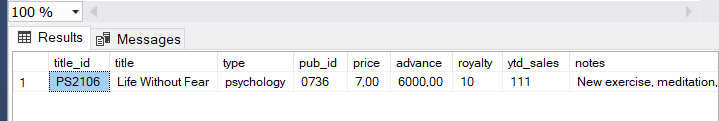
\includegraphics[width=0.9\linewidth]{Pic/lab4/SQ9.PNG}
    \caption{Выдача результата объединения двух таблиц для PS2106.}
    \label{fig:SQ9}
\end{figure}

Совместим все использованные команды. Ожидаемо результат будет как на рисунке \ref{fig:COcom}. Здесь мы использовали также инструкцию INNER JOIN, то есть включение одной таблицы в другую по принципу пересечения, и указали по какому атрибуту через ON. 

\begin{verbatim}
        SELECT t.title_id, stor_id, qty*price FROM titles t
        INNER JOIN sales ON t.title_id = sales.title_id
        WHERE t.title_id = 'PS2106'
\end{verbatim}
\begin{figure}[h!]
    \centering
    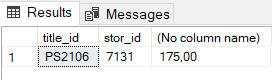
\includegraphics[width=0.5\linewidth]{Pic/lab4/SQ10.PNG}
    \caption{Выданный запрос.}
    \label{fig:COcom}
\end{figure}

Похожие запросы есть для операций объединения. Посмотрим следующий запрос. Операция LEFT OUTER JOIN объединяет операции в таблице titles (левой), дополняя строчки значениями из таблицы sales, где находит совпадения по атрибуту title\_id. Для строчек, у которых нет соответсвующей строчки в sales, заполняет значениями NULL (рис. \ref{fig:LEFT OUTER}).

\begin{verbatim}
        SELECT t.title_id, stor_id, qty*price FROM titles t
        LEFT OUTER JOIN sales ON t.title_id = sales.title_id
\end{verbatim}


Аналогичная операция для объединения в таблице sales (правой). Она соответсвует операции !A || (A \& B). Если же не указан параметр перед OUTER, тогда объединение произойдёт по принципу A || B. 
\begin{verbatim}
        SELECT t.title_id, stor_id, qty*price FROM titles t
        RIGHT OUTER JOIN sales ON t.title_id = sales.title_id
\end{verbatim}

\begin{figure}[h!]
    \centering
    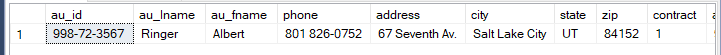
\includegraphics[width=0.9\linewidth]{Pic/lab4/SQ12.PNG}
    \caption{Объединение по принципу A \& B \& C.}
    \label{fig:ABC}
\end{figure}

Теперь попробуем выполнить предыдущие команды вместе. Результат на рисунке \ref{fig:ABC}. На нём представлено объединение всех таблиц по title\_id и au\_id.
\begin{verbatim}
        SELECT * FROM authors 
        INNER JOIN titleauthor
        INNER JOIN titles
        ON titleauthor.title_id = titles.title_id
        ON authors.au_id = titleauthor.au_id
        WHERE titles.title_id = 'PS2106'
\end{verbatim}
\begin{figure}[h!]
    \centering
    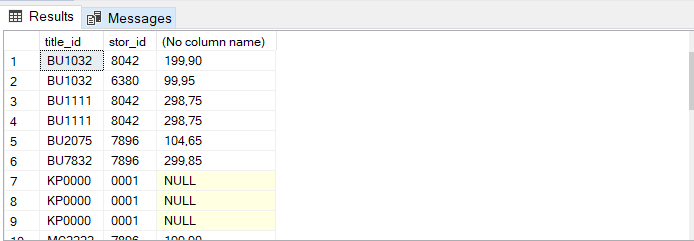
\includegraphics[width=0.9\linewidth]{Pic/lab4/SQ11.PNG}
    \caption{Операция !B || (A \& B).}
    \label{fig:LEFT OUTER}
\end{figure}

Следующая команда, с которой мы ознакомимся это DISTINCT. Она удаляет дубликаты из таблиц.

\begin{verbatim}
        SELECT DISTINCT au_id FROM titleauthor
\end{verbatim}

Также существует метод COUNT(), который считает количество ненулевых строчек. Инструкция * передаёт все атрибуты таблицы, когда обычно требуется указать отдельный столбец.

\begin{verbatim}
        SELECT COUNT(*) FROM titleauthor
\end{verbatim}

Теперь попробуем объединить две команды. DISTINCT удаляет дубликаты, а COUNT(*) посчитает кокличество записей. Очевидно, в счётчике нет дубикатов, так что DISCTINCT, по сути, бесполезен.
\begin{verbatim}
        SELECT DISTINCT COUNT(*) FROM titleauthor
\end{verbatim}

Если мы хотим посчитать количество уникальных строк, то надо действовать иначе. Сначала выполним DISTINCT, а потом результат передадим в метод COUNT().

\begin{verbatim}
        SELECT COUNT(DISTINCT au_id) FROM titleauthor.
\end{verbatim}

Этот запрос уже будет работать правильно. Сначала DISTINCT удалит дубликаты, а уже потом COUNT посчитает записи. Таким образом, получится количество уникальных записей.

Теперь разберёмся с системными таблицами. Дело в том, что через систему можно обратиться к таблице. По стандарту мы делали это через конструкцию USE. Но можно и через sys. Мы обратимся ко всем атрибутам, хранимым в БД запросом sys.columns. В нём есть атрибут name, который хранит имена атрибутов таблиц. Аналогично для названий самих таблиц. Результат запроса доступен на рисунке \ref{fig:SYSNAMEATR}. 

\begin{verbatim}
        SELECT sys.columns.name, sys.tables.name 
        FROM sys.columns
        INNER JOIN sys.tables
        ON sys.columns.object_id = sys.tables.object_id
\end{verbatim}

\begin{figure}[h!]
    \centering
    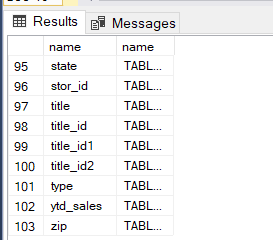
\includegraphics[width=0.3\linewidth]{Pic/lab4/SQ13.PNG}
    \caption{Имена таблиц и атрибутов.}
    \label{fig:SYSNAMEATR}
\end{figure}

Вместо sys.columns есть устаревшая конструкция syscolumns, которая несколько не вписывается в принцип инкапсуляции. Для этих запросов доступны все те же самые операции, что и для обычных SELECT-конструкций. Всю информацию, добытую в предыдущих командах, можно получить в виде общей схемы из INFORMATION\_SCHEMA.COLUMNS (рис. \ref{fig:INFSCHEMA}). 

\begin{verbatim}
        SELECT * FROM INFORMATION_SCHEMA.COLUMNS        
\end{verbatim}

\begin{figure}[h!]
    \centering
    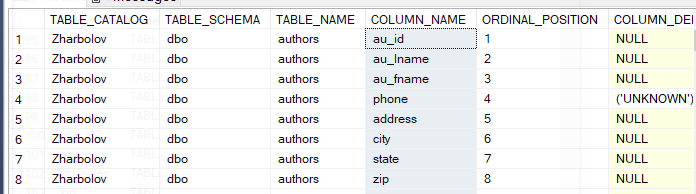
\includegraphics[width=0.9\linewidth]{Pic/lab4/SQ14.PNG}
    \caption{Схема атрибутов, их параметров и таблиц.}
    \label{fig:INFSCHEMA}
\end{figure}

Также существует таблица sysusers. Она хранит информацию обо всех акторах, имеющих доступ к таблицам БД.
\begin{figure}
    \centering
    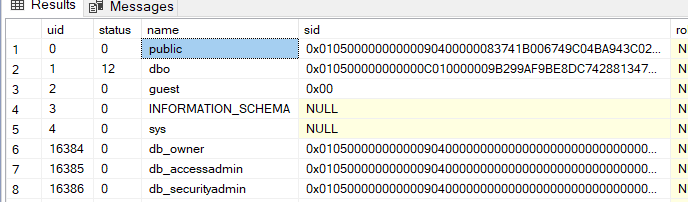
\includegraphics[width=0.9\linewidth]{Pic/lab4/SQ15.PNG}
    \caption{Таблица пользователей и акторов.}
    \label{fig:INFSCHEMT}
\end{figure}

На рисунке \ref{fig:INFSCHEMT} таблица sysusers. Здесь можно заметит различные типы доступа к БД: public, sys и, что примечательно, сама INFORMATION\_SCHEMA.

Далее разберёмся подбробнее с разнличными модификациями стандартной конструкции SELECT.

\begin{verbatim}
        SELECT title_id, ytd_sales, 
            'advance x2' = advaance*2, 'sum' = price*ytd_sales
        FROM titles
        WHERE advance*2 > ytd_sales*price
\end{verbatim}

Такие конструкции мы уже встречали, единственное новенькое здесь - это использование производных атрибутов для составления логических функций. Мы сравниваем удвоенный аванс с доходами от продаж: требуется, чтобы удвоенный аванс был больше. 

\begin{verbatim}
        SELECT title_id, ytd_sales, price*ytd_sales
        FROM titles
        WHERE ytd_sales between 4095 and 12000
\end{verbatim}

Здесь встречается новая логическая конструкция between. Она аналогична и заменяет следующую конструкцию: x1 <= A AND A <= x2. 

\begin{verbatim}
        SELECT id=au_id, name=au_lname, state=state
        FROM authors
        WHERE state not between 'CA' and 'IN'
\end{verbatim}

Этот запрос включает в себя наименования столбцов, а также показывает, что between умеет сравнивать не только в числовом диапазоне, но и лексикографически. Ещё используется логический оператор NOT.

\begin{verbatim}
        SELECT id_au_id, name=au_lname, state=state
        FROM authors
        WHERE state in ('CA', 'IN', 'MD')
\end{verbatim}

Предыдущий запрос показывает нам python-подобный синтаксис. Ключевое слово in - вхождение в массив. Конструкция state in... проверяет вхождение state в массив.

\begin{verbatim}
        SELECT id=au_id, name=au_lname, phone=phone
        FROM authors
        WHERE phone not like '415%'
\end{verbatim}

Эта конструкция демонстрирует нам использованный ранее синтаксис регулярных выражений через ключевое слово like. Мы видим выражение "415\%", что буквально означает, что телефон начинается с 415, а дальше что угодно.  

\begin{verbatim}
        SELECT id=au_id, name=au_lname, phone=phone
        FROM authors
        WHERE phone like '[2-7]1[2-9]%'
\end{verbatim}

Здесь представлено другое регулярное выражение. Конструкция проверяет, что телефон соответсвует шаблону: любая цифра от 2 до 7, 1, любая цифра от 2 до 9, затем что угодно. 

\begin{verbatim}
        SELECT title_id, type, advance
        FROM titles
        WHERE advance is NULL
\end{verbatim}

На этой конструкции появляется ещё один логический оператор, правда необычный. Он проверяет равенство, но равенство полное. В java для различий между равенством и тождественностью использовали оператора =, ==, ===. Зато в python используется подобный оператор is. Он проверяет являются ли объекты объектами одного типа, равными друг другу. В данном случае идёт проверка на тип NULL. Аналогично можно проверить на NOT NULL.

Наконец посмотрим команды, про которые упоминалось ранее. Мы можем данные не только доставать через SELECT, но и добавлять их в другие таблицы.

\begin{verbatim}
        SELECT title_id, title INTO NEW_TABLE FROM titles
\end{verbatim}

Попрактикуемся выполним следуюшие задания:
\begin{enumerate}
    \item Подсчитать количество изданий, в написании которых принял участие автор Карпов или Малыхин.
\begin{verbatim}
        SELECT COUNT(*)
        FROM authors
        WHERE au_fname in ('Карпов', 'Малыхина')

\end{verbatim}
    \item Вывод всех сведений об авторах изданий, опубликованных с 1997 г. по 1999 г.
\begin{verbatim}
        SELECT * FROM authors 
        INNER JOIN titleauthor
        INNER JOIN titles
        ON titleauthor.title_id = titles.title_id
        ON authors.au_id = titleauthor.au_id
        WHERE pubdate between '01/01/97' and '31/12/99'
\end{verbatim}
    \item Вывод всех сведений о продажах изданий, содержащих в названии слова "Psychology".
\begin{verbatim}
        SELECT * FROM authors 
        INNER JOIN titleauthor
        INNER JOIN titles
        ON titleauthor.title_id = titles.title_id
        ON authors.au_id = titleauthor.au_id
        WHERE CHARINDEX('Psychology', titles.title) > 0
\end{verbatim}
    \item Подсчитать общее количество изданий.
\begin{verbatim}
        SELECT COUNT(DISCTINCT title_id)
        FROM sales
\end{verbatim}
\end{enumerate}
\subsection{Вывод}
В ходе данной работы мы научились выполнять простейшие SQL-запросы, обращаться к атрибутам таблиц, смотреть их параметры и доставать их из системы.
\newpage
\section{Дополнительная информация}
\subsection{\centering Восстановительный скрипт для sp\_dboption}
\label{CODE:sp_dboption}
\begin{verbatim}
USE [master]
GO
SET ANSI_NULLS ON
GO

SET QUOTED_IDENTIFIER ON
GO

CREATE procedure [dbo].[sp_dboption]    -- 1999/08/09 18:25
    @dbname sysname = NULL,            -- database name to change
    @optname varchar(35) = NULL,        -- option name to turn on/off
    @optvalue varchar(10) = NULL        -- true or false
as
    set nocount on
    
    declare @dbid int            -- dbid of the database
    declare @catvalue int        -- number of category option
    declare @optcount int        -- number of options like @optname
    declare @allstatopts int    -- bit map off all options stored in sysdatqabases.status
                                -- that can be set by sp_dboption.
    declare @alloptopts int        -- bit map off all options stored in sysdatqabases.status
                                -- that can be set by sp_dboption.
    declare @allcatopts int        -- bit map off all options stored in sysdatqabases.category
                                -- that can be set by sp_dboption.
    declare @exec_stmt nvarchar(max)
    declare @fulloptname varchar(35)
    declare @alt_optname varchar(50)
    declare @alt_optvalue varchar(30)
    declare @optnameIn varchar(35)


    select @optnameIn = @optname
            ,@optname = LOWER (@optname collate Latin1_General_CI_AS)
            
    -- If no @dbname given, just list the possible dboptions.
    -- Only certain status bits may be set or cleared by sp_dboption.
    
    -- Get bitmap of all options that can be set by sp_dboption.
    select @allstatopts=number from master.dbo.spt_values where type = 'D'
        and name = 'ALL SETTABLE OPTIONS'
    select @allcatopts=number from master.dbo.spt_values where type = 'DC'
        and name = 'ALL SETTABLE OPTIONS'
    select @alloptopts=number from master.dbo.spt_values where type = 'D2'
        and name = 'ALL SETTABLE OPTIONS'

    if @dbname is null
    begin
        select 'Settable database options:' = name
            from master.dbo.spt_values
            where (type = 'D'
                and number & @allstatopts <> 0
                and number not in (0,@allstatopts)) -- Eliminate non-option entries
            or (type = 'DC'
                and number & @allcatopts <> 0
                and number not in (0,@allcatopts))
            or (type = 'D2'
                and number & @alloptopts <> 0
                and number not in (0,@alloptopts))
            order by name
        return (0)
    end

        -- Verify the database name and get info
        select @dbid = dbid
            from master.dbo.sysdatabases
            where name = @dbname

        -- If @dbname not found, say so and list the databases.
    if @dbid is null
    begin
        raiserror(15010,-1,-1,@dbname)
        print ' '
        select 'Available databases:' = name
            from master.dbo.sysdatabases
        return (1)
    end

    -- If no option was supplied, display current settings.
    if @optname is null
    begin
        select 'The following options are set:' = v.name
            from master.dbo.spt_values v, master.dbo.sysdatabases d
            where d.name=@dbname
                    and ((number & @allstatopts <> 0
                        and number not in (-1,@allstatopts)
                        and v.type = 'D'
                        and (v.number & d.status)=v.number)
                    or (number & @allcatopts <> 0
                        and number not in (-1,@allcatopts)
                        and v.type = 'DC'
                        and d.category & v.number <> 0)
                    or (number & @alloptopts <> 0
                        and number not in (-1,@alloptopts)
                        and v.type = 'D2'
                        and d.status2 & v.number <> 0))
        return(0)
    end

    if @optvalue is not null and lower(@optvalue) not in ('true', 'false', 'on', 'off')
    begin
        raiserror(15241,-1,-1)
        return (1)
    end

    -- Use @optname and try to find the right option.
    -- If there isn't just one, print appropriate diagnostics and return.
    select @optcount = count(*) ,@fulloptname = min(name)
        from master.dbo.spt_values
        where lower(name collate Latin1_General_CI_AS) like '%' + @optname + '%'
            and ((type = 'D'
                and number & @allstatopts <> 0
                and number not in (-1,@allstatopts))
            or (type = 'DC'
                and number & @allcatopts <> 0
                and number not in (-1,@allcatopts))
            or (type = 'D2'
                and number & @alloptopts <> 0
                and number not in (-1,@alloptopts)))
                
    -- If no option, show the user what the options are.
    if @optcount = 0
    begin
        raiserror(15011,-1,-1,@optnameIn)
        print ' '
        
        select 'Settable database options:' = name
            from master.dbo.spt_values
            where (type = 'D'
                    and number & @allstatopts <> 0
                    and number not in (-1,@allstatopts)) -- Eliminate non-option entries
                or (type = 'DC'
                    and number & @allcatopts <> 0
                    and number not in (-1,@allcatopts))
                or (type = 'D2'
                    and number & @alloptopts <> 0
                    and number not in (-1,@alloptopts))
            order by name

        return (1)
    end

    -- If more than one option like @optname, show the duplicates and return.
    if @optcount > 1
    begin
        raiserror(15242,-1,-1,@optnameIn)
        print ' '

        select duplicate_options = name
        from master.dbo.spt_values
        where lower(name collate Latin1_General_CI_AS) like '%' + @optname + '%'
            and ((type = 'D'
                and number & @allstatopts <> 0
                and number not in (-1,@allstatopts))
            or (type = 'DC'
                and number & @allcatopts <> 0
                and number not in (-1,@allcatopts))
            or (type = 'D2'
                and number & @alloptopts <> 0
                and number not in (-1,@alloptopts))
            )
        return (1)
    end

    -- Just want to see current setting of specified option.
    if @optvalue is null
    begin
        select OptionName = v.name,
            CurrentSetting = (case
                when ( ((v.number & d.status) = v.number
                        and v.type = 'D')
                    or (d.category & v.number <> 0
                        and v.type = 'DC')
                    or (d.status2 & v.number <> 0
                        and v.type = 'D2')
                    )
                    then 'ON'
                when not
                    ( ((v.number & d.status) = v.number
                        and v.type = 'D')
                    or (d.category & v.number <> 0
                        and v.type = 'DC')
                    or (d.status2 & v.number <> 0
                        and v.type = 'D2')
                    )
                    then 'OFF'
                end)
            from master.dbo.spt_values v, master.dbo.sysdatabases d
            where d.name=@dbname
                and ((v.number & @allstatopts <> 0
                    and v.number not in (-1,@allstatopts) -- Eliminate non-option entries
                    and v.type = 'D')
                or (v.number & @allcatopts <> 0
                    and v.number not in (-1,@allcatopts) -- Eliminate non-option entries
                    and v.type = 'DC')
                or (v.number & @alloptopts <> 0
                    and v.number not in (-1,@alloptopts) -- Eliminate non-option entries
                    and v.type = 'D2')
                    )
                and lower(v.name) = lower(@fulloptname)

        return (0)
    end

    select @catvalue = 0
    select @catvalue = number
            from master.dbo.spt_values
            where lower(name) = lower(@fulloptname)
            and type = 'DC'

    -- if setting replication option, call sp_replicationdboption directly
    if (@catvalue <> 0)
    begin
        select @alt_optvalue = (case lower(@optvalue)
                when 'true' then 'true'
                when 'on' then 'true'
                else 'false'
            end)

        select @alt_optname = (case @catvalue
                when 1 then 'publish'
                when 2 then 'subscribe'
                when 4 then 'merge publish'
                else quotename(@fulloptname, '''')
            end)

        select @exec_stmt = quotename(@dbname, '[') + '.dbo.sp_replicationdboption'
        EXEC @exec_stmt @dbname, @alt_optname, @alt_optvalue
        return (0)
    end


    -- call Alter Database to set options

    -- set option value in alter database
    select @alt_optvalue = (case lower(@optvalue)
            when 'true' then 'ON'
            when 'on' then 'ON'
            else 'OFF'
        end)
    -- set option name in alter database
    select @fulloptname = lower(@fulloptname)
    select @alt_optname = (case @fulloptname
            when 'auto create statistics' then 'AUTO_CREATE_STATISTICS'
            when 'auto update statistics' then 'AUTO_UPDATE_STATISTICS'
            when 'autoclose' then 'AUTO_CLOSE'
            when 'autoshrink' then 'AUTO_SHRINK'
            when 'ansi padding' then 'ANSI_PADDING'
            when 'arithabort' then 'ARITHABORT'
            when 'numeric roundabort' then 'NUMERIC_ROUNDABORT'
            when 'ansi null default' then 'ANSI_NULL_DEFAULT'
            when 'ansi nulls' then 'ANSI_NULLS'
            when 'ansi warnings' then 'ANSI_WARNINGS'
            when 'concat null yields null' then 'CONCAT_NULL_YIELDS_NULL'
            when 'cursor close on commit' then 'CURSOR_CLOSE_ON_COMMIT'
            when 'torn page detection' then 'TORN_PAGE_DETECTION'
            when 'quoted identifier' then 'QUOTED_IDENTIFIER'
            when 'recursive triggers' then 'RECURSIVE_TRIGGERS'
            when 'default to local cursor' then 'CURSOR_DEFAULT'
            when 'offline' then (case @alt_optvalue when 'ON' then 'OFFLINE' else 'ONLINE' end)
            when 'read only' then (case @alt_optvalue when 'ON' then 'READ_ONLY' else 'READ_WRITE' end)
            when 'dbo use only' then (case @alt_optvalue when 'ON' then 'RESTRICTED_USER' else 'MULTI_USER' end)
            when 'single user' then (case @alt_optvalue when 'ON' then 'SINGLE_USER' else 'MULTI_USER' end)
            when 'select into/bulkcopy' then 'RECOVERY'
            when 'trunc. log on chkpt.' then 'RECOVERY'
            when 'db chaining' then 'DB_CHAINING'
            else @alt_optname
        end)

    if @fulloptname = 'dbo use only'
    begin
        if @alt_optvalue = 'ON'
        begin
            if databaseproperty(@dbname, 'IsSingleUser') = 1
            begin
                raiserror(5066,-1,-1);
                return (1)
            end
        end
        else
        begin
            if databaseproperty(@dbname, 'IsDBOOnly') = 0
                return (0)
        end
    end

    if @fulloptname = 'single user'
    begin
        if @alt_optvalue = 'ON'
        begin
            if databaseproperty(@dbname, 'ISDBOOnly') = 1
            begin
                raiserror(5066,-1,-1);
                return (1)
            end
        end
        else
        begin
            if databaseproperty(@dbname, 'IsSingleUser') = 0
                return (0)
        end
    end

    select @alt_optvalue = (case @fulloptname
        when 'default to local cursor' then (case @alt_optvalue when 'ON' then 'LOCAL' else 'GLOBAL' end)
        when 'offline' then ''
        when 'read only' then ''
        when 'dbo use only' then ''
        when 'single user' then ''
        else @alt_optvalue
    end)

    if lower(@fulloptname) = 'select into/bulkcopy'
    begin
        if @alt_optvalue = 'ON'
        begin
            if databaseproperty(@dbname, 'IsTrunclog') = 1
                select @alt_optvalue = 'RECMODEL_70BACKCOMP'
            else
                select @alt_optvalue = 'BULK_LOGGED'
        end
        else
        begin
            if databaseproperty(@dbname, 'IsTrunclog') = 1
                select @alt_optvalue = 'SIMPLE'
            else
                select @alt_optvalue = 'FULL'
        end
    end
    if lower(@fulloptname) = 'trunc. log on chkpt.'
    begin
        if @alt_optvalue = 'ON'
        begin
            if databaseproperty(@dbname, 'IsBulkCopy') = 1
                select @alt_optvalue = 'RECMODEL_70BACKCOMP'
            else
                select @alt_optvalue = 'SIMPLE'
        end
        else
        begin
            if databaseproperty(@dbname, 'IsBulkCopy') = 1
                select @alt_optvalue = 'BULK_LOGGED'
            else
                select @alt_optvalue = 'FULL'
        end
    end

    -- construct the ALTER DATABASE command string
    select @exec_stmt = 'ALTER DATABASE ' + quotename(@dbname) + ' SET ' + @alt_optname + ' ' + @alt_optvalue + ' WITH NO_WAIT'
    EXEC (@exec_stmt)

    if @@error <> 0
    begin
        raiserror(15627,-1,-1)
        return (1)
    end

    return (0) -- sp_dboption
GO

\end{verbatim}

\subsection{\centering Описание таблиц и их полей для Лабораторной работы №2}

Таблица \textbf{authors} — авторы. Поля таблицы authors:
\begin{enumerate}
\label{DB2INFO}
\item \textbf{au\_id} — уникальный идентификатор (первичный ключ) записи об авторе, представленный в формате номера полиса социального страхования. Формат поля имеет вид: ХХХ-ХХ-ХХХХ, где Х десятичная цифра от 0 до 9, - — знак «минус» в номере полиса. Поле является первичным ключом таблицы, имеет тип VARCHAR(11) и должно соответствовать (проверяться сервером) заданному формату;

\item \textbf{au\_Iname} — фамилия автора, тип VARCHAR(40). Не допускает отсутствия значения (NOT NULL);

\item \textbf{au\_fname} — имя автора, тии VARCHAR(20). Не допускает отсутствия значения (NОТ NULL);

\item \textbf{phone} — номер телефона автора, тип CHAR(12), NОТ NULL, имеет умалчиваемое значение 'UNKNOWN';

\item \textbf{address} — адрес, тип VARCHAR(40). Значение адреса может быть не задано
(NULL);

\item \textbf{city} — город VARCHAR(20), может быть нe задан (NULL);

\item \textbf{state} — штат, в котором проживает автор. Задается двухсимвольной аббревиатурой (например, CA), может быть не задан (NULL);

\item \textbf{zip} — почтовый индекс из 5 десятичных цифр. Формат поля имеет вид: ХХХХХ, где X десятичная цифра от 0 до 9. В БД должно контролироваться соответствие данных заданному формату. Допускается отсутствие значения данного в поле;

\item \textbf{contract} — битовое (Bit) поле, означающее наличие или отсутствие контракта с автором. Не допускает отсутствия значения (NOT NULL).
\end{enumerate}

Таблица \textbf{titles} — печатные издания, авторы которых перечислены в предыдущей таблице. Поля таблицы titles:
\begin{enumerate}
\item \textbf{title\_id} - уникальное 6-ти символьное поле. Образует первичный ключ таблицы Titles. Первые два символа буквы, остальные — десятичные цифры,

\item \textbf{tithe} — название книги VARCHAR(80), обязательное для ввода (NOT NULL);

\item \textbf{type} — тип (область знаний) издания, например, business. Строковые значения CHAR (12). Не допускает отсутствия значения (МОТ NULL). Имеет умалчиваемое значение ‘UNDECIDED ' - неизвестно;

\item \textbf{pub\_id} — поле, являющееся ссылкой на запись в таблице «Издательство», которая не представлена в данной базе, CHAR (4), NULL;

\item \textbf{price} — цена книги, MONEY, NULL;

\item \textbf{advance} — сумма аванса, выданная автору (авторам), MONEY, NULL;

\item \textbf{royalty} — авторский гонорар (в процентах), INT, NULL;

\item \textbf{ytd\_sales} — количество проданных экземпляров издания, INT, NULL;

\item \textbf{notes} — примечание, VARCHAR(200), NULL;

\item \textbf{pubdate} — дата, когда издание было подписано и передано в печать. Тип DATETIME. Требует обязательного ввода (NOT NULL). По умолчанию должна сохраняться дата создания записи DEFAULT (getdate()).
\end{enumerate}

Таблица \textbf{titleauthor} обеспечивает связь «многие ко многим» между записями таблицы authors и таблицы titles для этого она имеет поля au\_id и title\_id, являющиеся внешними ключами. Поля таблицы titleauthor:

\begin{enumerate}

\item \textbf{au\_id} — внешний ключ, ссылающийся на первичный ключ таблицы Authors. Поэтому, поле может принимать значения, 
 представленные в столбце au\_id таблицы Authors. Требует обязательного ввода, имеет тип и формат столбца au\_id таблицы Authors;

\item \textbf{title\_id} - внешний ключ, ссылающийся на первичный ключ таблицы Titles. Поле может принимать значения, представленные в столбце title\_id таблицы Titles. Требует обязательного ввода, имеет тип и формат столбца title\_id таблицы Titles;

\item \textbf{au\_ord} — порядковый номер автора, заданного au\_id в списке соавторов книги, заданной title id. Имеет тип TINYINT, может не имеет значения (свойство NULL);

\item \textbf{royaltype} — процент авторского гонорара, принадлежащего этому конкретному автору за написание этой книги. Тип INT, NULL. 


Значения полей (au\_id, title\_id) являются уникальными и образуют первичный ключ таблицы titleauthor.
\end{enumerate}

Таблица \textbf{sales} — список продаж (поставок) партий книг в магазины. Каждому изданию (книге) - в таблице titles может соответствовать несколько строк (поставленных партий экземпляров книги) в таблице Sales. Поля таблицы:

\begin{enumerate}
\item \textbf{stor\_id} - ссылка на записи в другой неиспользуемой в данной базе таблице. Тип CHAR(4), NOT NULL;

\item \textbf{ord\_num} — строковое данное VARCHAR(20), NOT NULL;

\item \textbf{ord\_date} — дата поставки партии экземпляров книги. Тип DATETIME, NOT NULL;

\item \textbf{qty} - количество экземпляров книги в данной партии. Тип SMALLINT, NOT NULL;

\item \textbf{payterms} — условия оплаты. Тип VARCHAR(12), NULL;

\item \textbf{title\_id} — внешний ключ, ссылающийся Ha первичный ключ таблицы Titles. Поле может принимать значения, представленные в столбце title\_id таблицы Titles. Требует обязательного ввода, имеет тип и формат столбца title\_id таблицы Titles.

Поля (stor\_id, ord\_num, title\_id) составляют первичный ключ таблицы Sales.
\end{enumerate}
\newpage
\subsection{Вставленные в таблицы данные}
\label{DATA3}
\begin{figure}[h!]
    \begin{minipage}[p]{0.45\linewidth}
        \centering
        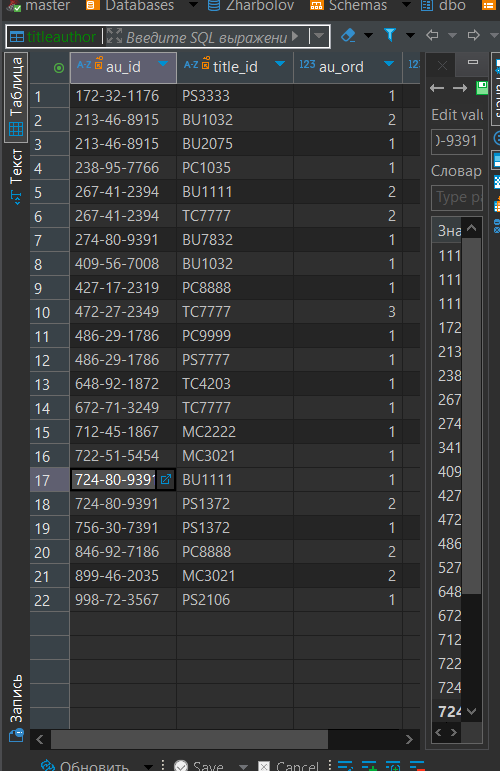
\includegraphics[width=0.8\linewidth]{Pic/lab3/DataTA.PNG}
        \caption{Таблица titleauthor.}
    \end{minipage}
    \hfill
    \begin{minipage}[p]{0.45\linewidth}
        \centering
        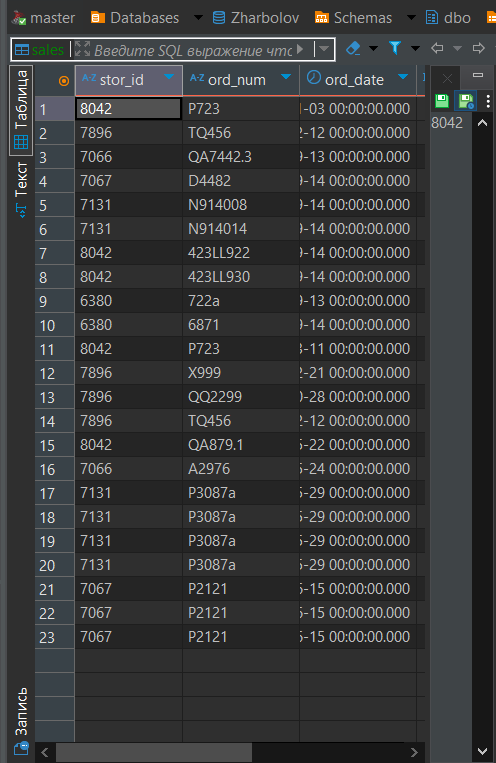
\includegraphics[width=0.8\linewidth]{Pic/lab3/DataSale.PNG}
        \caption{Таблица sales.}
    \end{minipage}
    
\end{figure}

\begin{figure}[h!]
    \begin{minipage}[p]{0.45\linewidth}
        \centering
        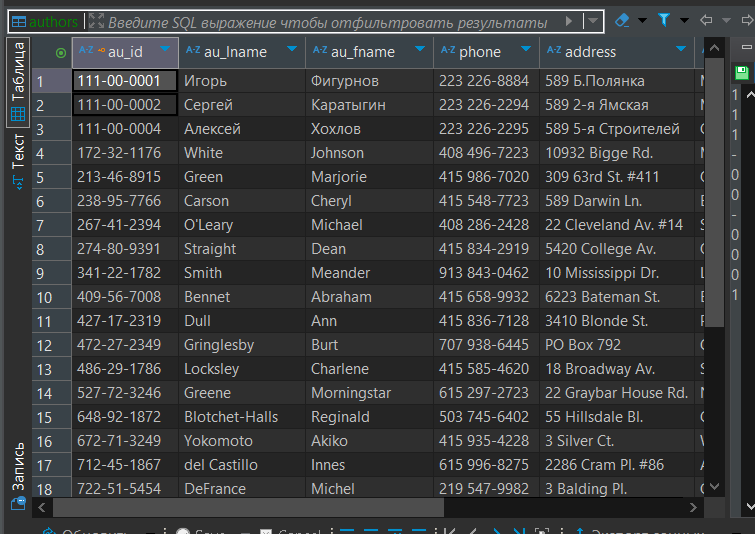
\includegraphics[width=0.8\linewidth]{Pic/lab3/DataAuthors.PNG}
        \caption{Таблица authors.}
    \end{minipage}
    \hfill
    \begin{minipage}[p]{0.45\linewidth}
        \centering
        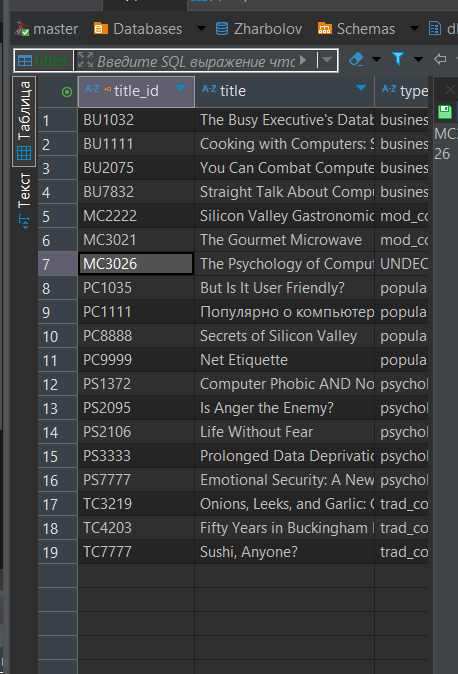
\includegraphics[width=0.8\linewidth]{Pic/lab3/DataTitle.PNG}
        \caption{Таблица titles.}
    \end{minipage}
    
\end{figure}


% Не редактируем: Страница библиографии (формируется автоматически из книжек, указанных в refs.bib и пометок \cite{имя_источника} в тексте)
\newpage
\printbibliography[title=Перечень использованных источников]
\addcontentsline{toc}{section}{Перечень использованных источников}
\end{document}
